%%%%%%%%%%%%%%%%%%%%%%%%%%%%%%%%%%%%%%%%%%%%%%%%%%%%%%%%%%%%%%%%%%%%%%%%
%                                                                      %
%     File: Thesis_Results.tex                                         %
%     Tex Master: Thesis.tex                                           %
%                                                                      %
%     Author: Andre C. Marta                                           %
%     Last modified : 29 Jan 2021                                      %
%                                                                      %
%%%%%%%%%%%%%%%%%%%%%%%%%%%%%%%%%%%%%%%%%%%%%%%%%%%%%%%%%%%%%%%%%%%%%%%%

\chapter{Collision-aware real-time \acrshort{nmpc} over irregular terrain}
\label{chapter:obstacleAvoidance}

This chapter takes on the \acrshort{nmpc} algorithm developed in the previous chapter, and reformulates it in order to prevent collisions and safeguard the vehicle safety. Firstly, the generation of a new and free of collisions reference is outlined in section \ref{section:saferefgen}. Then, this reference is fed to an one-stage \acrshort{ocp} that safeguards a minimum clearance of the position horizon to the nearest obstacle (section \ref{section:realtimesafenmpcroughterrain}). This chapter is mostly based on the work of \citet{schoels2020ciao, schoels2020nmpc}.

\begin{remark}
In this chapter, $\mathbf{p}_2$ is expressed by $\mathbf{p}$. 
\end{remark}

\section{Safe reference generation}
\label{section:saferefgen}

Some \acrshort{nmpc} applications rely on a nonconvex condition to keep the mobile away from collisions \cite{mpc_frenetserret}, like $d_\mathcal{O}\left(\mathbf{p}\right) \geq \underline{d}$. Although some interesting results are reported, this inequality constraint is not suitable for real-time applications \cite{schoels2020ciao}. On the other hand, the introduction of a map of minimum distances into the \acrshort{nmpc} also introduces excessive nonlinearities that prevent real-time feasibility.

Therefore, this chapter aims to simplify the problem by placing some operations outside the \acrshort{nmpc} and to convexify the clearance condition.

\subsection{\acrlong{ciao} (\acrshort{ciao}) algorithm}

On the road to generate a safe reference, one needs to compute the distance to the closest obstacle but also the direction that points to safe space positions away from the closest obstacle. In order to accomplish that, some definitions are laid out below, as well as the method that aims to find the biggest ball that contains $\mathbf{p}$ and is on safe space.

\begin{definition}[Distance function]
The distance function is defined as the euclidean distance at position $\mathbf{p}$ to the closest obstacle, such that $d_\ObstacleSpace:\Map_2 \rightarrow \mathbb{R}$.

\begin{equation}
d_\mathcal{\ObstacleSpace}\left(\mathbf{p}\right) = \underset{\mathbf{o} \in \mathcal{\ObstacleSpace}}{\text{min}}\;\| \mathbf{p} - \mathbf{o} \|_2
\end{equation}
\end{definition}

\begin{definition}[Safe space]
Let $\ObstacleSpace$ be the occupied space and $\underline{d} > 0$ the safety margin. Then, the safe space $\mathcal{\SafeSpace}$ is defined as,

\begin{equation}
\mathcal{\SafeSpace} = \{\mathbf{p}_2 \in \Map_2: d_\ObstacleSpace\left(\mathbf{p}\right) \geq \underline{d} \}
\end{equation}
\end{definition}

Then, a safe ball around $\mathbf{c} \in \SafeSpace$ is defined that includes $\mathbf{p}$. This safe ball is not centered in $\mathbf{p}$, because if $\mathbf{p}$ is too close to $\ObstacleSpace$, the size of the safe ball is small. Due to that, a bigger safe ball is required so that more space of maneuver is given to the solver (figure \ref{fig:freeballs}). Therefore, the optimization problem (7) of \cite{schoels2020ciao} is employed to find $\SafeSpace_\mathbf{c}$.

\begin{figure}[!htb]
	\centering
	\begin{subfigmatrix}{3}
	\subfigure[$ \|\mathbf{p} - \mathbf{o}\|_2^2 \leq \left(d_\ObstacleSpace\left(\mathbf{p}\right) - \underline{d}\right)^2$] {
	\begin{tikzpicture}
		\node (A) at (0, 2.0) {};
		\node (B) at (-0.5, 2.0) {};
		\node (C) at (-0.5, -0.4) {};
		\node (D) at (0.0, -0.4) {};
		\node (E) at (-1.0, -0.4) {};
		\fill[pattern = north east lines] (0, 0) rectangle (0.32, 3.5);
		\draw[line width=1pt] (0.0, 0.0) -- (0, 3.5);
		\draw[dashed, line width=0.5pt] (-0.5, -0.4) -- (-0.5, 3.5);
		\draw[->] (A.center) -- node[midway, above] {$\underline{d}$} (B.center);
		\draw[->] (C) -- node[midway, above] {$\overline{\SafeSpace}$} (D);
		\draw[->] (C) -- node[midway, above] {$\SafeSpace$} (E);
		\filldraw[black] (-1.5, 1.8) circle (2pt) node[anchor=east]{$\mathbf{p}$};
		\draw (-1.5, 1.8) circle (1.0);
	\end{tikzpicture}
	}
	\subfigure[$\SafeSpace_\mathbf{c}$] {
	\begin{tikzpicture}
		\node (A) at (0, 2.0) {};
		\node (B) at (-0.5, 2.0) {};
		\node (C) at (-0.5, -0.4) {};
		\node (D) at (0.0, -0.4) {};
		\node (E) at (-1.0, -0.4) {};
		\node (Pb) at (-1.5, 1.8) {};
		\node (Cb) at (-2.8, 1.8) {};
		\fill[pattern = north east lines] (0, 0) rectangle (0.32, 3.5);
		\draw[line width=1pt] (0.0, 0.0) -- (0, 3.5);
		\draw[dashed, line width=0.5pt] (-0.5, -0.4) -- (-0.5, 3.5);
		\draw[->] (A.center) -- node[midway, above] {$\underline{d}$} (B.center);
		\draw[->] (C) -- node[midway, above] {$\overline{\SafeSpace}$} (D);
		\draw[->] (C) -- node[midway, above] {$\SafeSpace$} (E);
		\filldraw[black] (-1.5, 1.8) circle (1.0pt) node[anchor=north]{$\mathbf{p}$};
		\filldraw[black] (-2.8, 1.8) circle (1.0pt) node[anchor=north]{$\mathbf{c}$};
		\draw (-2.8, 1.8) circle (2.3);
		\draw[->] (Pb) -- node[midway, above] {$\eta \cdot \mathbf{g} + \mathbf{p}$} (Cb);
		\node (Fs) at (-4.8, 1.8) {$\SafeSpace_\mathbf{c}$};
	\end{tikzpicture}
	}
	\subfigure[$\mathbf{g}$ (\textcolor{blue}{blue arrows}); Filled black circles are obstacles.] {
	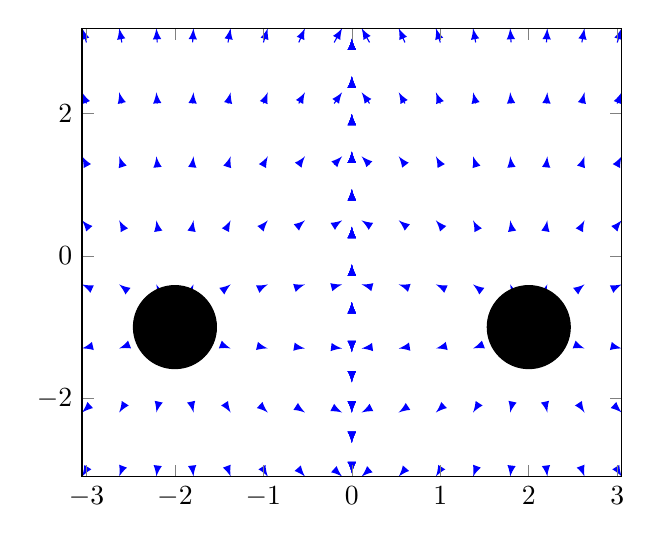
\begin{tikzpicture}
		\begin{axis}[
    		view={0}{90},        % top-down view
    		domain=-3:3,
    		y domain=-3:3,
		]
 		\addplot3[
  			blue,
    		quiver={u=x+2, v=y+1, scale arrows=0.05},
    		samples=8,
    		-latex,
    		domain=-3:-0.2,
    		y domain=-3:3] (x, y, 0);
    	\addplot3[
  			blue,
    		quiver={u=x-2, v=y+1, scale arrows=0.05},
    		samples=8,
    		-latex,
    		domain=0.2:3,
    		y domain=-3:3] (x, y, 0);
    	\addplot3[
  			blue,
    		quiver={u=0, v=1, scale arrows=0.05},
    		samples=8,
    		-latex,
    		domain=-3:3,
    		y domain=-0.7:3] (0, y, 0);
    	\addplot3[
  			blue,
    		quiver={u=0, v=-1, scale arrows=0.05},
    		samples=5,
    		-latex,
    		domain=-3:3,
    		y domain=-3:-1.3] (0, y, 0);
		\filldraw[black] (-2, -1) circle (15.0pt){};
		\filldraw[black] (2, -1) circle (15.0pt){};
		\end{axis}
	\end{tikzpicture}
	}
	\end{subfigmatrix}
	\caption{Type of free balls and distance function normalized gradient.}
    \label{fig:freeballs}
\end{figure}
	
\begin{definition}[Safe ball]
\begin{equation}
\SafeSpace_\mathbf{c} = \{\mathbf{p} \in \SafeSpace: \|\mathbf{p} - \mathbf{c} \|_2^2 \leq \left( d_\ObstacleSpace\left(\mathbf{c}\right) - \underline{d} \right)^2 \}
\end{equation}
\end{definition}

\acrlong{nlp} \eqref{eq:ciaomax} sums up the optimization problem (7) of \cite{schoels2020ciao}. The search direction is also defined to be the normalized gradient of the distance function with respect to the updated circle center $\mathbf{c}$ at every iteration. The step $\eta$ is upper bounded in order to avoid high computation times. The reader is advised to read \cite{schoels2020ciao, schoels2020nmpc} for an in-depth explanation of the theoretical framework the \acrshort{ciao} algorithm is based on.
\begin{subequations}\label{eq:ciaomax}
\begin{gather}
	\underset{\eta}{\text{max}} \hspace{1mm} \eta \label{subeq:ciaoproblem}\\
	\text{subject to} \hspace{5mm} \underline{\eta} \leq \eta \leq \overline{\eta},\; \underline{\eta} > 0 \label{subeq:etaconstraints}\\
	d_\ObstacleSpace( \underbrace{\eta \cdot \mathbf{g} + \mathbf{p} }_{\mathbf{c}^*}) = \eta + d_\ObstacleSpace\left( \mathbf{p} \right) \label{subeq:ciaoconstraint}\\
	\mathbf{g} = \frac{\nabla d_\ObstacleSpace\left(\mathbf{p}\right)}{\|\nabla d_\ObstacleSpace\left(\mathbf{p}\right)\|_2}
	\label{subeq:searchdirection}
\end{gather}
\end{subequations}
\subsubsection*{Implementation}

\acrshort{nlp} \eqref{eq:ciaomax} is solved by employing a line search problem. Let $\ObstacleSpace_i \subset \Map_2$ be a subset of obstacles that make $\ObstacleSpace$, such that $\ObstacleSpace = \bigcup\limits_{i} \ObstacleSpace_i$. For the sake of simplicity, only static, circled obstacles are considered.

To some position $\mathbf{p}$, the distance to $\ObstacleSpace_i$ is computed. Then, the distance function is equal to the distance to the closest obstacle, such that $d_\ObstacleSpace\left(\mathbf{p}\right) = \text{min} \left(d_{\ObstacleSpace_i}\left(\mathbf{p}\right)\right)$. Then, $\nabla d_\ObstacleSpace\left(\mathbf{p}\right)$ is determined by computing the normalized vector that connects $\mathbf{p}$ to the closest obstacle. In case there is more than one obstacle with a distance to $\mathbf{p}$ that equals $d_\ObstacleSpace\left(\mathbf{p}\right)$, $\mathbf{g}$ becomes the normalized vector of the sum of the vectors that connect $\mathbf{p}$ to the respective obstacle, such that $\mathbf{g} = \frac{\sum_{\mathbf{o} \in \underline{\ObstacleSpace}} \mathbf{p} - \mathbf{o}}{\|\sum_{\mathbf{o} \in \underline{\ObstacleSpace} } \mathbf{p} - \mathbf{o}\|}$, where $\underline{\ObstacleSpace} \subset \ObstacleSpace$ denotes the set of closest obstacles to $\mathbf{p}$. The right side picture of figure \ref{fig:freeballs} depicts this explanation. At the middle line between both obstacles, one can see that the direction of $\mathbf{g}$ changes dramatically, because the gradient becomes the normalized sum of the arrows that connect $\mathbf{p}$ to each obstacle along this line.

Finally, the step $\eta$ is consecutively increased by multiplying it by some factor $\delta_{\eta} > 1$ until the constraints \eqref{subeq:etaconstraints} and \eqref{subeq:ciaoconstraint} are not respected.

\begin{algorithm}[H]
	\caption{\footnotesize \textsc{GETSAFEBALL}}\label{alg:computefreespace}
	\centering
	\footnotesize
	\begin{algorithmic}[1]
	\Function{getsafeballcenter}{$\underline{\eta},\,\overline{\eta},\,\delta_{\eta},\,\mathbf{p},\,d_\ObstacleSpace\left(\cdot\right),\,\nabla d_\ObstacleSpace\left(\cdot\right)$}
	\State $\eta \gets \underline{\eta}$ \Comment{initialize $\eta$}
	\State $\mathbf{c} \gets \mathbf{p}$ \Comment{initial ball center}
	\State $d_\ObstacleSpace\left(\mathbf{c}\right) \gets \text{min} \left(d_{\ObstacleSpace_i}\left(\mathbf{c}\right)\right)$
	\State $\mathbf{g} \gets \frac{\sum_{\mathbf{o} \in \underline{\ObstacleSpace}} \mathbf{c} - \mathbf{o}}{\|\sum_{\mathbf{o} \in \underline{\ObstacleSpace} } \mathbf{c} - \mathbf{o}\|}$
	\While{$\eta \leq \overline{\eta}$ and \eqref{subeq:ciaoconstraint} stand}
	\State $\mathbf{c} \gets \eta \cdot \mathbf{g} + \mathbf{c}$ \Comment{update ball center}
	\State $d_\ObstacleSpace\left(\mathbf{c}\right) \gets \text{min} \left(d_{\ObstacleSpace_i}\left(\mathbf{c}\right)\right)$
	\State $\eta \gets \eta \times \delta_{\eta}$
	\EndWhile
	\State \Return $\mathbf{c}^* \gets \mathbf{c}$
	\EndFunction
	\end{algorithmic}
\end{algorithm}
	
\subsubsection*{Results}

The results of the application of algorithm \nameref{alg:computefreespace} are presented in figure \ref{fig:ciaoiterationresults}, where the occupied area is the one where $\ObstacleSpace = \{\mathbf{p} \in \Map_2:d_\ObstacleSpace\left(\mathbf{p}\right)\leq0\}$.

\begin{figure}[!htb]
  \begin{subfigmatrix}{2}
    \subfigure[$d_\ObstacleSpace\left(\cdot\right)$ and $\mathbf{g}$ (black arrows)]{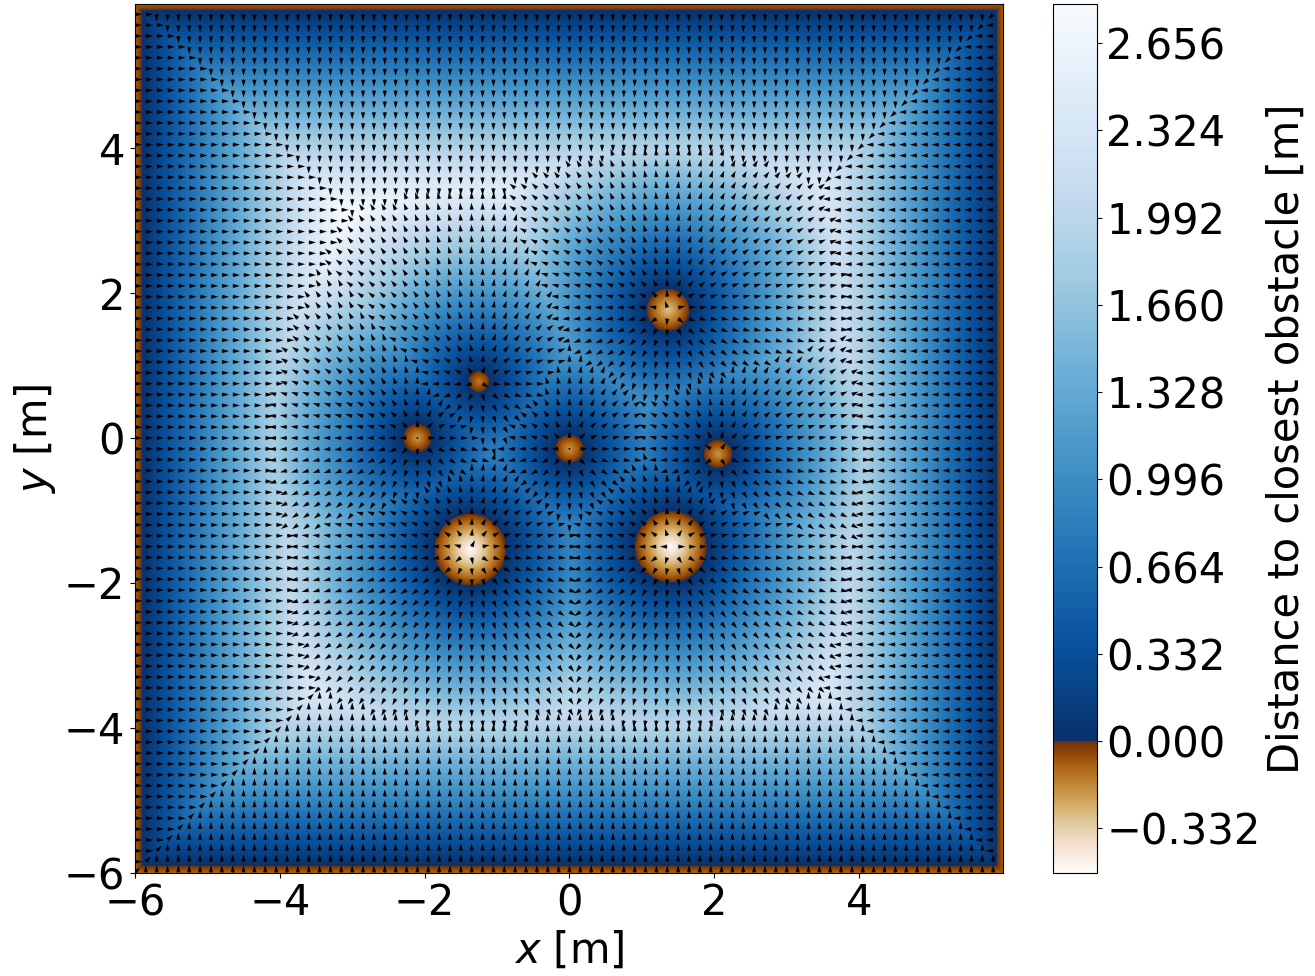
\includegraphics[width=0.49\linewidth]{Figures/Obstacle avoidance/CIAO/d2o_gradient_d2o.png}}
    \subfigure[Examples of safe balls, where $\mathbf{c}$ and $\mathbf{p}$ are denoted by $\bullet$ and $\mathbf{\times}$, respectively.]{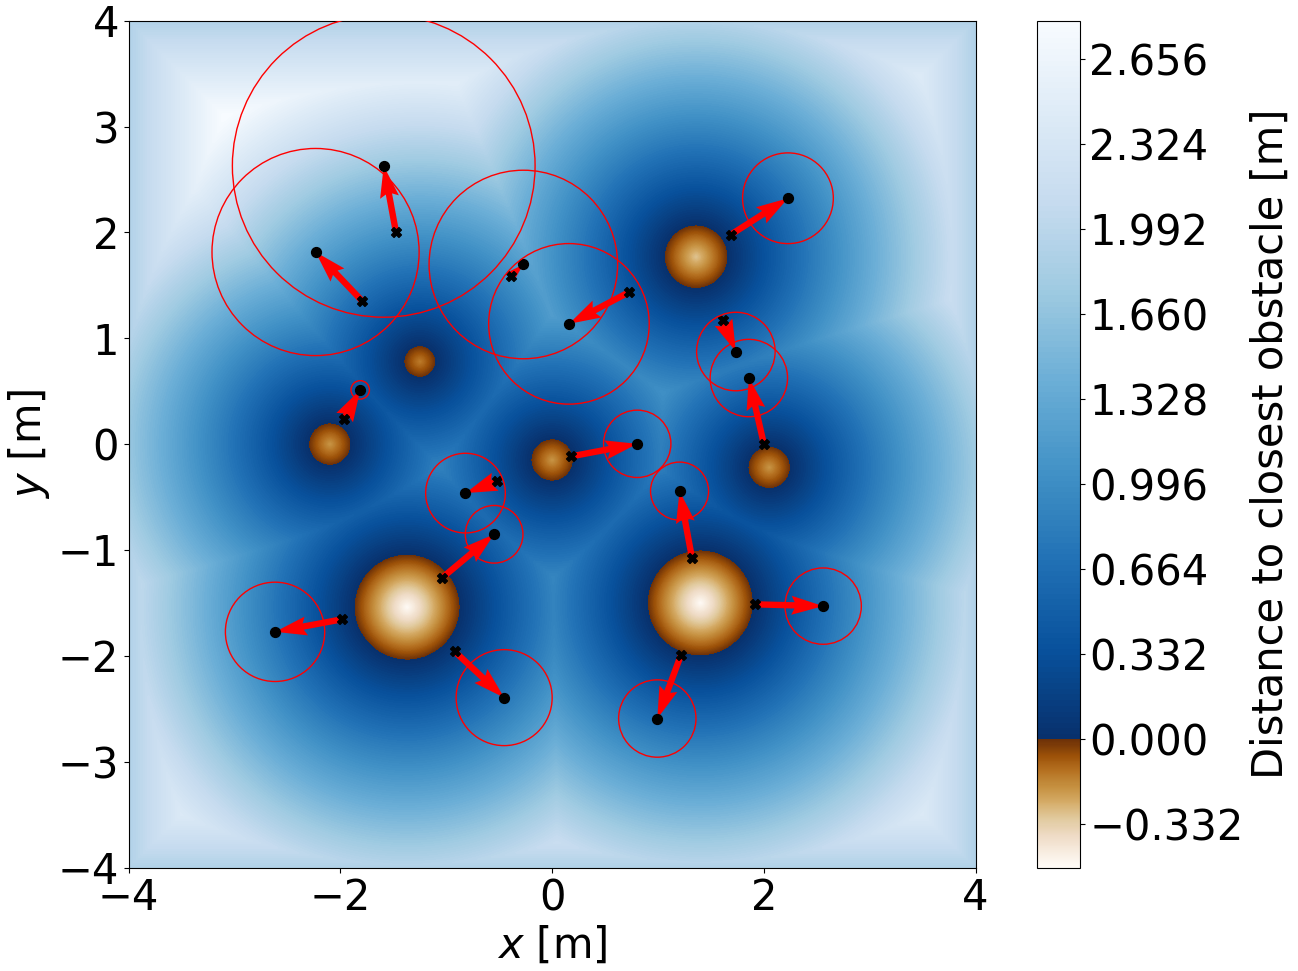
\includegraphics[width=0.49\linewidth]{Figures/Obstacle avoidance/CIAO/ciao_iteration_test.png}}
  \end{subfigmatrix}
  \caption{Application of algorithm \nameref{alg:computefreespace} to a set of obstacles, where $\underline{\eta} = 0.02,\,\overline{\eta} = 2.0,\,\delta_{\eta} = 2.0$ and $\underline{d} = 0.3$.}
  \label{fig:ciaoiterationresults}
\end{figure}

In case $\mathbf{p}$ is such that $d_\ObstacleSpace\left(\mathbf{p}\right)\geq \underline{d}$, algorithm \nameref{alg:computefreespace} ensures $\mathbf{p} \in \SafeSpace_{\mathbf{c}}$. The right picture of figure \ref{fig:ciaoiterationresults} shows proof that $\SafeSpace_{\mathbf{c}}$ stops expanding either when $\eta$ reaches its maximum or when \refeq{subeq:ciaoconstraint} fails. Finally, algorithm \nameref{alg:computefreespace} was run for 629 different positions $\mathbf{p}$ with the same conditions as the ones that generated the right picture of \ref{fig:ciaoiterationresults}. The maximum recorded computation time was $0.1\,ms$.

\subsection{Baseline reference deformation}

Algorithm \nameref{alg:computefreespace} can be used to project points of the baseline reference $\mathbf{r}$ that belong to $\overline{\SafeSpace}$ into the nearest safe space position. Then a look-ahead target position, $\mathbf{t} \in \SafeSpace$, in the projected reference is defined. The deformed reference is generated with respect to this point.

In order to meet that end, an artificial potential field is generated with respect to each obstacle and the target. The target radiates an attractive field whereas the obstacles radiate a repulsive field \cite{chapter47handbookrobotics}.
\begin{subequations}\label{eq:potentialfield}
\begin{gather}
	\mathbf{f}_{att}\left(\mathbf{t},\,\mathbf{p}\right) = k_{att}\,	\frac{\mathbf{t} - \mathbf{p}}{\|\mathbf{t}-\mathbf{p}\|} \label{subeq:atractivefield} \\
	\mathbf{f}_{rep}\left(\mathbf{p},\,\ObstacleSpace\right) = \begin{cases}
	k_{rep}\, \sum\limits_{\mathbf{o}\in\ObstacleSpace} \left(\frac{1}{\|	\mathbf{p} - \mathbf{o}\|_2-r_\mathbf{o}} - \frac{1}{d_0}\right)\frac{\mathbf{p} - \mathbf{o}}{\|\mathbf{p}-\mathbf{o}\|}\;&\text{if}\;\|\mathbf{p} - \mathbf{o}\|_2-r_\mathbf{o} < d_0\\
	0\;&\text{if}\;\|\mathbf{p} - \mathbf{o}\|_2-r_\mathbf{o} \geq d_0
\end{cases}\label{subeq:repulsivefield}
\end{gather}
\end{subequations}

Equation \eqref{eq:potentialfield} presents the set of atractive and repulsive fields, where $k_{att}$ and $k_{rep}$ are parameters that regulate the importance of each potential. Then, the total potential at $\mathbf{p}$ is expressed by the sum of all potentials, such that $\mathbf{f}_{tot} = \mathbf{f}_{att} + \mathbf{f}_{rep}$. Every potential exerts a radial field. Each repulsive field \eqref{subeq:repulsivefield} only exerts a force up to $d_0$ from the border of each obstacle. This repulsive field decreases dramatically as $\|\mathbf{p} - \mathbf{o}\|_2-r_\mathbf{o}$ approaches $d_0$.

Then, one may generate a deformed reference by selecting a target $\mathbf{t} \in \SafeSpace$ that is \textbf{always} at a minimum distance of $d_s$ to the closest obstacle when its projection is required. Then, from a position $\mathbf{p} \in \SafeSpace$ one may generate a deformed reference that aims to reach $\mathbf{t}$, where $\mathbf{r}_{def} \subset \SafeSpace$ denotes the vectors of poses of the deformed reference along the \acrshort{nmpc} horizon.

\subsubsection*{Implementation}

Based on the current position $\mathbf{p}$ of the mobile robot, a look-ahead target is defined, so that there is considerable distance between both positions. From the first reference position, the next positions are consecutively defined based on the potential field direction at the respective position. The euclidean distance between consecutive positions is also defined so that velocity bounds are respected.

Unfortunately, artificial potential fields have local minimums. In case the reference generation falls into one of these spots, the reference gets trapped there. Fast marching methods solve this issue but these methods are not suitable for real-time use, because the computation of the Eikonal equation solution is a big computational overhead.

Apart from the target, local minimums are close to obstacles, where repulsive and attractive fields cancel each other. From trial and error, these positions may be avoided by selecting look-ahead targets that are not close to the vehicle configuration. On the other hand, if the look-ahead target is too far away, the same issue may come up. Algorithm \nameref{alg:gendeformedref} sums up the explanation laid out in the last three paragraphs. 

\begin{algorithm}[H]
	\caption{\footnotesize \textsc{GETDEFORMEDREF}}\label{alg:gendeformedref}
	\centering
	\footnotesize
	\begin{algorithmic}[1]
		\Function{getdeformedreference}{$\mathbf{p},\,\mathbf{r},\,d_\ObstacleSpace\left(\cdot\right),\,\nabla d_\ObstacleSpace\left(\cdot\right),\,\ObstacleSpace,\,N,\,v,\,\alpha,\,\alpha_+,\,d_s,\,k_{rep},\,k_{att}$}
	\State $\mathbf{t}\gets\mathbf{r}\left(\alpha+\alpha_+\right)$ \Comment{get look-ahead target}
	\If{$d_\ObstacleSpace\left(\mathbf{t}\right) < d_s$}
		\State $\mathbf{t}_{proj} \gets \mathbf{t} + \mathbf{g}(\mathbf{t}) \cdot \left(d_s - d_\ObstacleSpace(\mathbf{t})\right)$ \Comment{project $\mathbf{t}$ to a close safe space point}
	\Else	
		\State $\mathbf{t}_{proj}\gets\mathbf{t}$
	\EndIf
	\State $k \gets 0$
	\State $\mathbf{r}_{def,\,k} \gets\mathbf{p}$
	\While{$k \leq N$}
		\If{$\mathbf{r}_{def,\,k} \not\in \neighborhood(\mathbf{t}_{proj})$} \Comment{update reference till reference approaches target neighbourhood}
			\State $\mathbf{r}_{def,\,k + 1} \gets \mathbf{r}_{def,\,k} + \mathbf{f}_{tot}\left(\mathbf{t},\,\mathbf{r}_{def,\,k},\,\ObstacleSpace\right)\,v$ \Comment{get deformed reference from potential field}
		\Else
			\State $\mathbf{r}_{def,\,k + 1} \gets \mathbf{r}_{def,\,k}$ \Comment{fill reference with last reference pose}
		\EndIf
		\State $k \gets k+1$	
	\EndWhile
	\State \Return $\mathbf{r}_{def}$
	\EndFunction
	\end{algorithmic}
\end{algorithm}

In algorithm \nameref{alg:gendeformedref}, $\alpha$ denotes the closest baseline reference position locator, whereas $\alpha_+$ expresses the locator difference from $\alpha$ to the look-ahead target in the baseline reference. When the deformed reference reaches the projected target neighbourhood $\neighborhood(\mathbf{t}_{proj})$, the empty reference nodes are filled with the last updated deformed reference pose.

\subsubsection*{Results}

Figure \ref{fig:potentialfieldresults} presents the visual results of the application of algorithm \nameref{alg:gendeformedref} to the same set of obstacles from figure \ref{fig:ciaoiterationresults}. Although the deformed reference successfully deviates from $\ObstacleSpace$, it still crosses $\overline{\SafeSpace}$. This is not necessarily an issue as the most important safety metric is to make sure that the mobile robot position and its horizon is always in $\SafeSpace$.

Algorithm \nameref{alg:gendeformedref} was also run 3029 times and the recorded average and maximum run times were $0.36\;ms$ and $0.76\;ms$, respectively. In each of these simulations, it is mandatory that $\mathbf{p}\in\SafeSpace$, because it doesn't make sense to apply algorithm \nameref{alg:gendeformedref} to cases where $\mathbf{p}\in\overline{\SafeSpace}$, as the mobile robot hull touches $\ObstacleSpace$. The algorithm is suitable for real-time use.

\begin{figure}[!htb]
  \begin{subfigmatrix}{2}
    \subfigure[$\mathbf{f}_{tot}(\cdot)$, where $k_{rep}=0.2,\,k_{att}=3.0$ and $d_0=0.35$. The target is the \textcolor{tabred}{red} point and the obstacles are coloured in \textcolor{tabgray}{gray}. \textcolor{tabgreen}{Green} points denote local minimum spots, where $\mathbf{f}_{tot}(\cdot)=0$.]{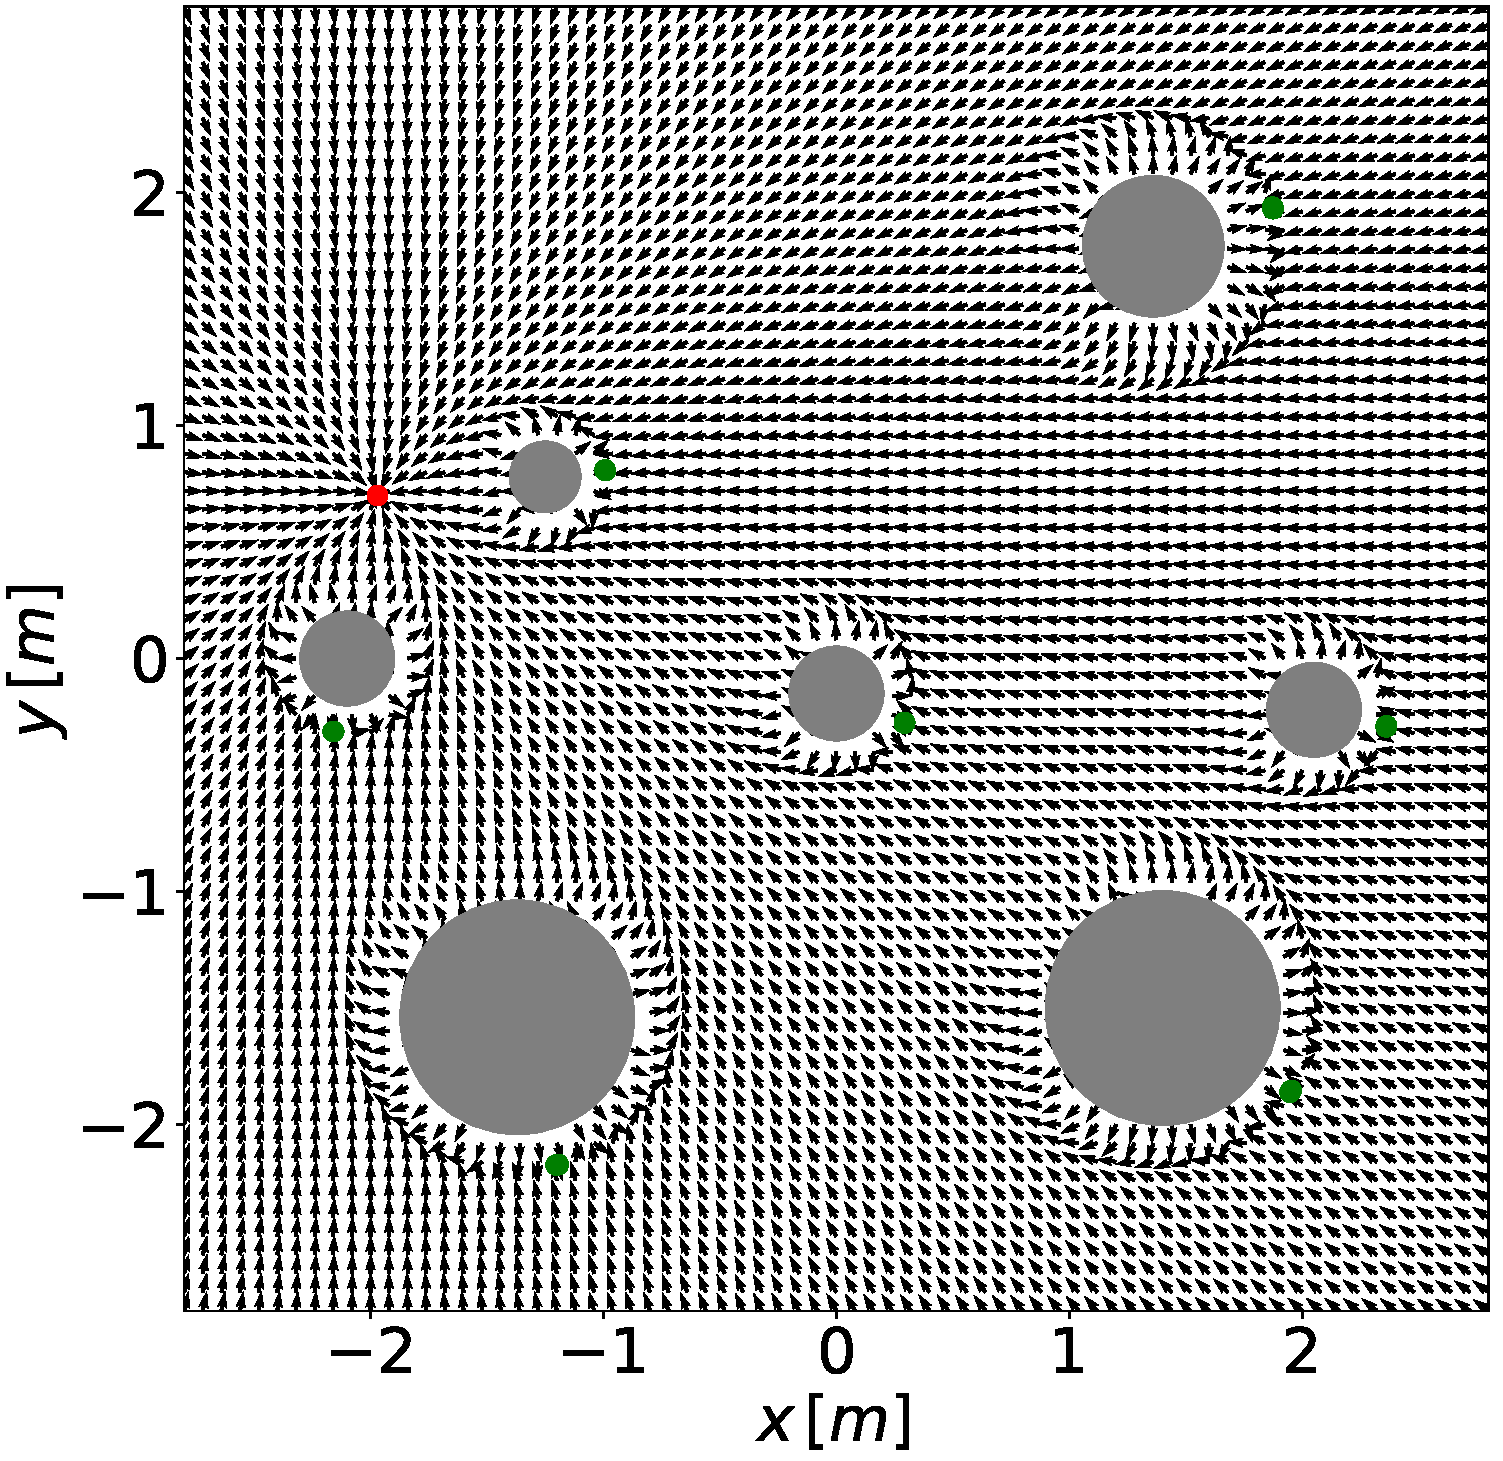
\includegraphics[width=0.49\linewidth]{Figures/Obstacle avoidance/Potential field/potential_field.pdf}}
    \subfigure[Examples of deformed references, where $N=50,\,v=0.02$, $\alpha_+=0.3$, $\underline{d} = 0.3$ and $d_s = 1.2 \times \underline{d}$. The target and respective reference have the same color. The target and projected target are marked with $\times$ and $\bullet$ respectively. Dashed \textcolor{tabgray}{gray} lines depict the border of $\overline{\SafeSpace}$.]{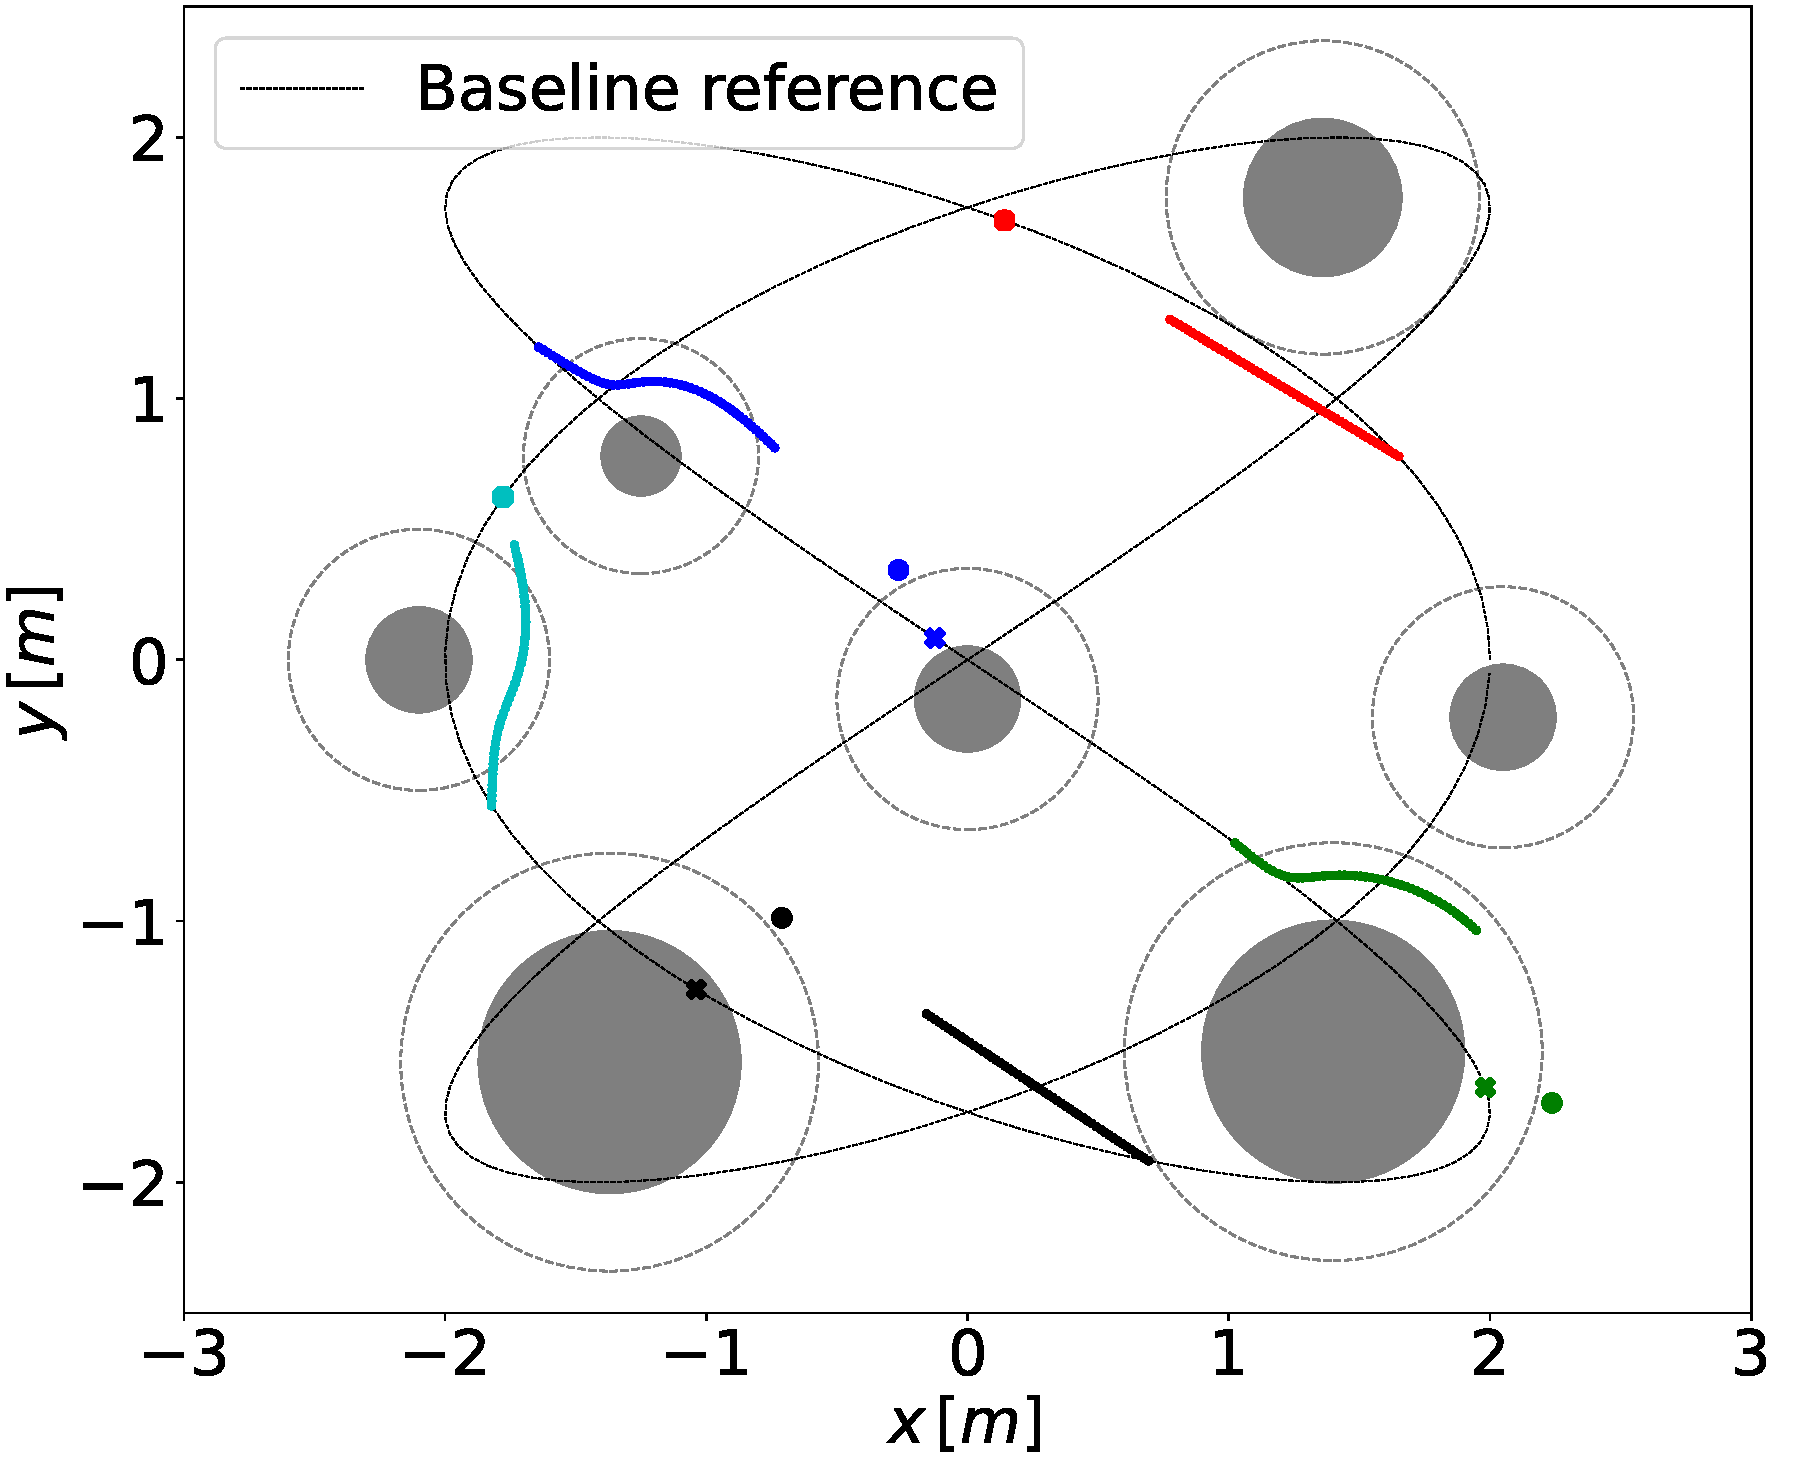
\includegraphics[width=0.49\linewidth]{Figures/Obstacle avoidance/Potential field/deformed_ref_examples.pdf}}
  \end{subfigmatrix}
  \caption{Application of algorithm \nameref{alg:gendeformedref} to a set of obstacles. The parameters that generated the results of figure \ref{fig:ciaoiterationresults} were used to generate these figures as well. The potential field parameters from the left picture were used to generate the right picture.}
  \label{fig:potentialfieldresults}
\end{figure}

\section{Real-time safe \acrshort{nmpc} over irregular terrain}
\label{section:realtimesafenmpcroughterrain}

Finally, it is possible to integrate algorithms \nameref{alg:computefreespace} and \nameref{alg:gendeformedref} into a real-time optimal control simulation, in order to safely guide the mobile robot away from $\overline{\SafeSpace}$. Once again, the \acrshort{nmpc} architecture is restructured to accomodate new constraints. Moreover, the \acrshort{nmpc} algorithm is also reformulated to include the algorithms described above. Figure \ref{fig:architecturesafenmpc} presents the new structure where the \acrshort{nmpc} is fed by a deformed reference and the safe balls $\SafeSpace_{\mathbf{c}^*}$ around each position of the problem's initial guess. Each of these safe balls define the area of admissable positions for each node, so that the next optimal position horizon doesn't enter $\overline{\SafeSpace}$.

\begin{figure}[!htb]
\centering
\tikzstyle{block} = [draw, text centered, minimum height = 2.0em, minimum width = 3.0em, rounded corners, line width = 0.5 mm]
	\begin{tikzpicture}
		\node [block, align = center] at (2.0, -1.3) (1) {\shortstack{Algorithm\\ \nameref{alg:determineeulerangles}}};
		\node [block, align = center, draw={rgb,255:red,30;green,145;blue,30}] at (-2.0, 0) (2) {\textcolor{rgb,255:red,30;green,145;blue,30}{Virtual speed control}};
		\node [block, align = center] at (2.0, 0.0)	(5) {\shortstack{Algorithm\\ \nameref{alg:gendeformedref}}};
		\node [block, align = center] at (2.0, 1.0)	(6) {\shortstack{Algorithm\\ \nameref{alg:computefreespace}}};
		\node [block, align = center] at (6.0, 0) (3) {NMPC\\Dynamics};
		\node [block, align = center] at (9.5, 0) (4) {Plant};
  		\draw [-latex, thick, align = center] (4)
  												 -- ++(1.0, 0.0)
  												 -- ++(0.0, -2.5)
  												 -- coordinate (bottomSeg) node [above, xshift=-2em] {$\mathbf{\hat{x}}_0$} ++(-14.5, 0.0)
  												 -- ++(0.0, 2.5)
  												 -- (2);				
    	\coordinate (pointBelow3) at ($(3 |- bottomSeg)$);
    	\coordinate (pointBelow2) at ($(2 |- bottomSeg)$);
    	\filldraw[black] (pointBelow3) circle (1pt);
    	\filldraw[black] (pointBelow2) circle (1pt);
  		\draw [-latex, thick, align=center] ([yshift=4.0]3.east)
		-- ++(0.3, 0.0)
		-- ++(0.0, 0.7) coordinate (fork)
		-- node[above] {$\mathbf{w}^*$} ++(-0.8, 0.0)
		-- (3);
		\filldraw[black] (fork) circle (1pt);
		\draw [-latex, thick, align=center] (1)
		-- node [above] {$\hat{\roll}_0,\,\hat{\pitch}_0$} ++(2.5, 0.0)
		-- (3);
  		\draw [-latex,thick] (2) -- node [above] {$\mathbf{r}$} (5);
  		\draw [-latex,thick] (5) -- node [above] {$\mathbf{r}_{def}$} (3);
  		\draw [-latex,thick] (3) -- node [above] {$\mathbf{u}_0^*$} (4);
  		\draw [-latex, thick] (pointBelow3) -- (3);
  		\draw [-latex, thick] (pointBelow2) -- ++ (0.0, 1.2) -- (1);
  		\draw [-latex, thick] (fork) -- ++ (0.0, 1.0) -- node [above] {$\mathbf{p}_2^*$} ++(-4.0, 0.0) -- (6);
  		\draw [-latex, thick] (6) -- ++ (2.0, 0.0) -- node [above] {$\SafeSpace_{\mathbf{c}^*}$} (3);
	\end{tikzpicture}
	\caption{Safe real-time \acrshort{nmpc} architecture.}
	\label{fig:architecturesafenmpc}
\end{figure}

The set of equations \eqref{eq:lagrangemayersafeocp} and \eqref{eq:safeonestageocp} define the cost terms and the linear and non-linear constraints of the new one-stage safe \acrshort{ocp}, respectively. Equation \eqref{subeq:ciaocirclesarea} is the new appended non-linear constraint. This constraint sets the admissable area for each position of the optimal horizon. $\mathbf{c}_k^*,\,d_\ObstacleSpace(\mathbf{c}_k^*)$ and $d_s$ are parameters of the problem that come from the results of algorithm \ref{alg:computefreespace}.

Secondly, another major novelty is the introduction of slacks. The need to relax constraint \ref{subeq:ciaocirclesarea} comes from the observation that the \acrshort{ocp} sometimes becomes infeasible if $\mathbf{p}_2^*$ is pushed to the border of $\SafeSpace_{\mathbf{c}^*}$. Slacks are non-negative (\ref{subeq:slackbounds}) and are also weighted on the cost function terms \ref{subeq:onestagelagrangesafeocp} and \ref{subeq:onestagemayersafeocp}. $Z_k \gg 1$ so that $s_k$ is only active when it is of the utmost importance to prevent infeasibility \cite{schoels2020nmpc}. $z_k$ penalizes very fast rates of change of $s_k$.
\begin{subequations}
\begin{gather}
\lagrangeTerm{\mathbf{\x},\,\mathbf{u},\,\mathbf{r}_{def},\,s}_k = \Vert\x - r_{\x,\,def},\,\y - r_{\y,\,def},\,e_{\yaw},\,\vx,\,\wz,\,\delta \Traction_l,\,\delta \Traction_r\Vert_{Q,\,k}^2 \; + \Vert u_l,\,u_r \Vert_{R,\,k}^2 + \frac{1}{2}\,s_k^2\,Z_k+ s_k\,z_k\label{subeq:onestagelagrangesafeocp}\\
\mayerTerm{\mathbf{\x},\,\mathbf{r}_{def},\,s}_k = \Vert\x - r_{\x,\,def},\,\y - r_{\y,\,def},\,e_{\yaw},\,\vx,\,\wz,\,\delta \Traction_l,\,\delta \Traction_r\Vert_{Q,\,k}^2 + \frac{1}{2}\,s_k^2\,Z_k+ s_k\,z_k\label{subeq:onestagemayersafeocp}
\end{gather}
\label{eq:lagrangemayersafeocp}
\end{subequations}
\vspace{-1.2cm}
\begin{subequations}
	\begin{gather}
		\underset{\mathbf{x}_k,\,\mathbf{u}_k,\,s_k}{\text{minimize}} \sum_{k=0}^{N-1} \lagrangeTerm{\mathbf{\x}_k,\,\mathbf{u}_k,\,\mathbf{r}_{k,\,def},\,s_k} + \mayerTerm{\mathbf{\x}_N,\,\mathbf{r}_{N,\,def},\,s_N} \label{subeq:costonestagesafeocp}\\
			\mathbf{x}_0 = \mathbf{\hat{x}}_0\\
			\DerMathBold{x}(t) = \processModel{\mathbf{x}(t), \mathbf{u}(t), \mathbf{p}} \tag{\ref{eq:skidsteeringStateSpace}}\\
			\left(m\,g\,\sin(\pitch_k)\,\frac{1}{4}+\delta\Traction_{l,\,k}\right)^2 + \left(m\,g\,\cos(\pitch_k)\,\sin(\roll_k)\,\frac{1}{4}\right)^2 - \left(\FrictionCoefficient\,m\,g\,\cos(\pitch_k)\,\cos(\roll_k)\,\frac{1}{4}\right)^2 \leq 0 \label{subeq:frictionconetlsafeocp}\\
			\left(m\,g\,\sin(\pitch_k)\,\frac{1}{4}+\delta\Traction_{r,\,k}\right)^2 + \left(m\,g\,\cos(\pitch_k)\,\sin(\roll_k)\,\frac{1}{4}\right)^2 - \left(\FrictionCoefficient\,m\,g\,\cos(\pitch_k)\,\cos(\roll_k)\,\frac{1}{4}\right)^2 \leq 0 \label{subeq:frictionconetrsafeocp}\\
			\|\mathbf{p}_k - \mathbf{c}_k^*\|_2^2 - (d_\ObstacleSpace(\mathbf{c}_k^*) - d_s)^2 \leq s_k \label{subeq:ciaocirclesarea}\\
			s_k \geq 0 \label{subeq:slackbounds}\\
			\begin{pmatrix}
			(v_x)_{min}\\
			(\omega_z)_{min}
			\end{pmatrix} \leq \begin{pmatrix}
			v_x\\
			\omega_z
			\end{pmatrix} \leq \begin{pmatrix}
			(v_x)_{max}\\
			(\omega_z)_{max}
			\end{pmatrix}
	\end{gather}
	\label{eq:safeonestageocp}
\end{subequations}

The list of states and controls remains unchanged. The slacks horizon, $\mathbf{s} = \left[s_0,\,s_1,\ldots,s_N\right]$, also becomes an optimization variable of the problem. Moreover, the set of parameters becomes $\mathbf{p} = \left[\FrictionCoefficient,\,m,\,g,\,\InertiaTensor_{zz},\,d_s,\,\mathbf{c}^*,\,d_\ObstacleSpace(\mathbf{c}^*),\,\mathbf{r}_{def}\right]$, where $\mathbf{c}^* = \left[\mathbf{c}_0^*,\,\mathbf{c}_1^*,\,\ldots,\,\mathbf{c}_N^*\right]$ encapsulates the list of the safe balls centers. Finally, $\mathbf{r}_{def} = \left[\x_0,\,\y_0,\,\yaw_0,\,\x_1,\,\y_1,\,\yaw_1,\,\ldots,\,\x_N,\,\y_N,\,\yaw_N\right]_{def}$. This one-stage safe \acrshort{ocp} preserves convexity as cost terms are all positive semi-definite and constraints are circles or linear intervals.

\subsection{Simultaneous path tracking and obstacle avoidance on rough terrain}

From now on, the results of the application of the safe \acrshort{ocp} are presented and discussed. Table \ref{tab:SafeRoughPathTrackingSpecs} denote the cost terms of the solvers that are tested in this subsection. Solver $(1)$ gives much less room for the slacks to increase than solver $(2)$. From this subsection to the end of the chapter, $d_s = \underline{d}$. The rest of the parameters are equal to the ones mentioned in figure \ref{fig:potentialfieldresults}. The heightmap and virtual speed control module are the same of subsection \ref{subsection:traversalRoughTerrain}.

\begin{table}[!htb]
  \caption[Safe \acrshort{ocp} cost terms and parameters.]{Safe \acrshort{ocp} cost terms and parameters($N = 40,\; T_s = 40\,ms$).}
  \label{tab:SafeRoughPathTrackingSpecs}
  \renewcommand{\arraystretch}{1.2}
  \centering
  \begin{tabular}[]{lcc}
	\toprule
	Solver & $(1)$ & $(2)$ \\
	\midrule
	$Q_i$ & $diag\left(3.0\times1.1^i,\,3.0\times1.1^i,\,3.0\times1.1^i,\,1\mathrm{e}{-9},\,1\mathrm{e}{-9},\,1\mathrm{e}{-9},\,1\mathrm{e}{-9}\right)$ & Same as $(1)$\\
	$R$ & $diag\left(1.0,\,1.0\right)$ & Same as $(1)$\\
	$Z_i$ & $1\mathrm{e}{6}$ & $1\mathrm{e}{3}$ \\
	$Z_N$ & $1\mathrm{e}{6}$ & $1\mathrm{e}{3}$ \\
	$z_i$ & $1.0$ & Same as $(1)$ \\
	$z_N$ & $1.0$ & Same as $(1)$ \\
  	\bottomrule
  \end{tabular}
  \begin{tabular}[]{cccccc}
  	\toprule
  		$\left[(v_x)_{min},\; (v_x)_{max}\right]\,[m/s]$ & $\left[(\omega_z)_{min},\; (\omega_z)_{max}\right]\,[rad/s]$ & $\left[(u_i)_{min},\,(u_i)_{max}\right]\,[N \cdot s]$ & $\FrictionCoefficient$ & $\sigma_{\roll}$ & $\sigma_{\pitch}$\\
  	\midrule
  		$\left[-5.0,\,5.0\right]$ & $\left[-5.0,\,5.0\right]$ & $\left[-100,\,100\right]$ & $0.7$ & $7\mathrm{e}{-2}$ & $7\mathrm{e}{-2}$\\
  	\bottomrule
  \end{tabular}
\end{table}

Figure \ref{fig:pathtrackingsafeocp} assembles the path tracking results of solver $(1)$ at different initial conditions. Reference tracking and obstacle avoidance is successfully achieved. The mobile robot also does not enter $\overline{\SafeSpace}$, but moves alongside the border at most. On top of the bottom left obstacle, the mobile robot turns around because the target is so far ahead that the potential field guides the deformed reference to the right, instead of circling the obstacle.

On the other hand, figure \ref{fig:reftoursolver2} presents path tracking results with solver $(2)$. In this case, the mobile robot enters $\overline{\SafeSpace}$. This happens because the weight that penalize the slacks is much smaller, which allows the slacks to be greater. Due to that, the solver expands the admissable area in such a way that there is a big intersection between \ref{subeq:ciaocirclesarea} and $\overline{\SafeSpace}$. It is clear that this solver configuration is undesirable as the mobile robot is placed on risky situations. Then, the purpose of slacks is to provide flexbility to the \acrshort{ocp}, in order to allow the mobile robot to briefly enter $\overline{\SafeSpace}$ so that infeasibility does not occur. The same problem was run without slacks and infeasibility typically happened when the circles are very small and the vehicle is at the border of the \acrshort{ciao} circles. 

\begin{figure}[!htb]
  \begin{subfigmatrix}{2}
    \subfigure[Reference tour with solver $(1)$.]{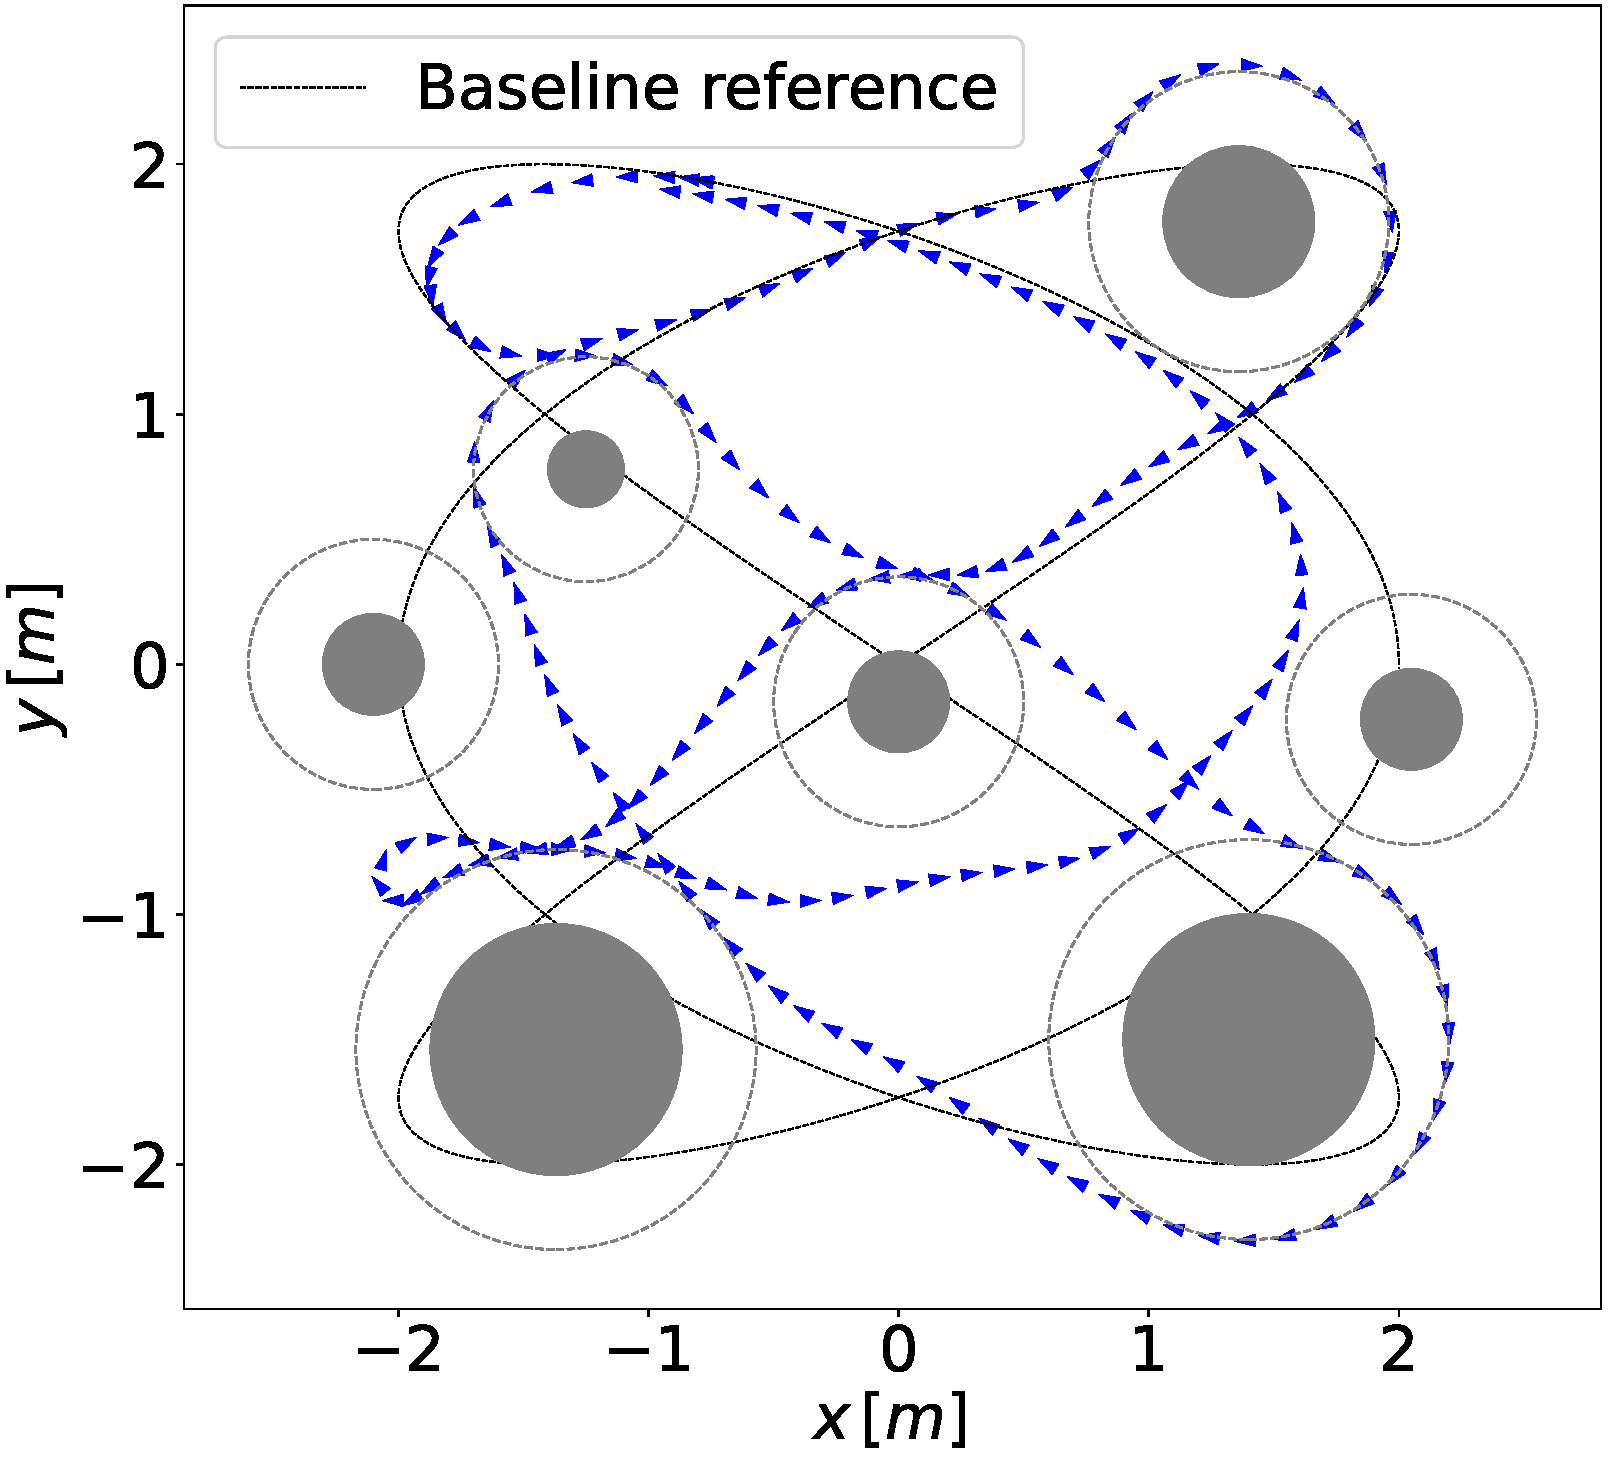
\includegraphics[width=0.49\linewidth]{Figures/Obstacle avoidance/Safe NMPC/tour_part1_solver_1.pdf}}
    \subfigure[Path tracking from different initial poses with solver $(1)$.]{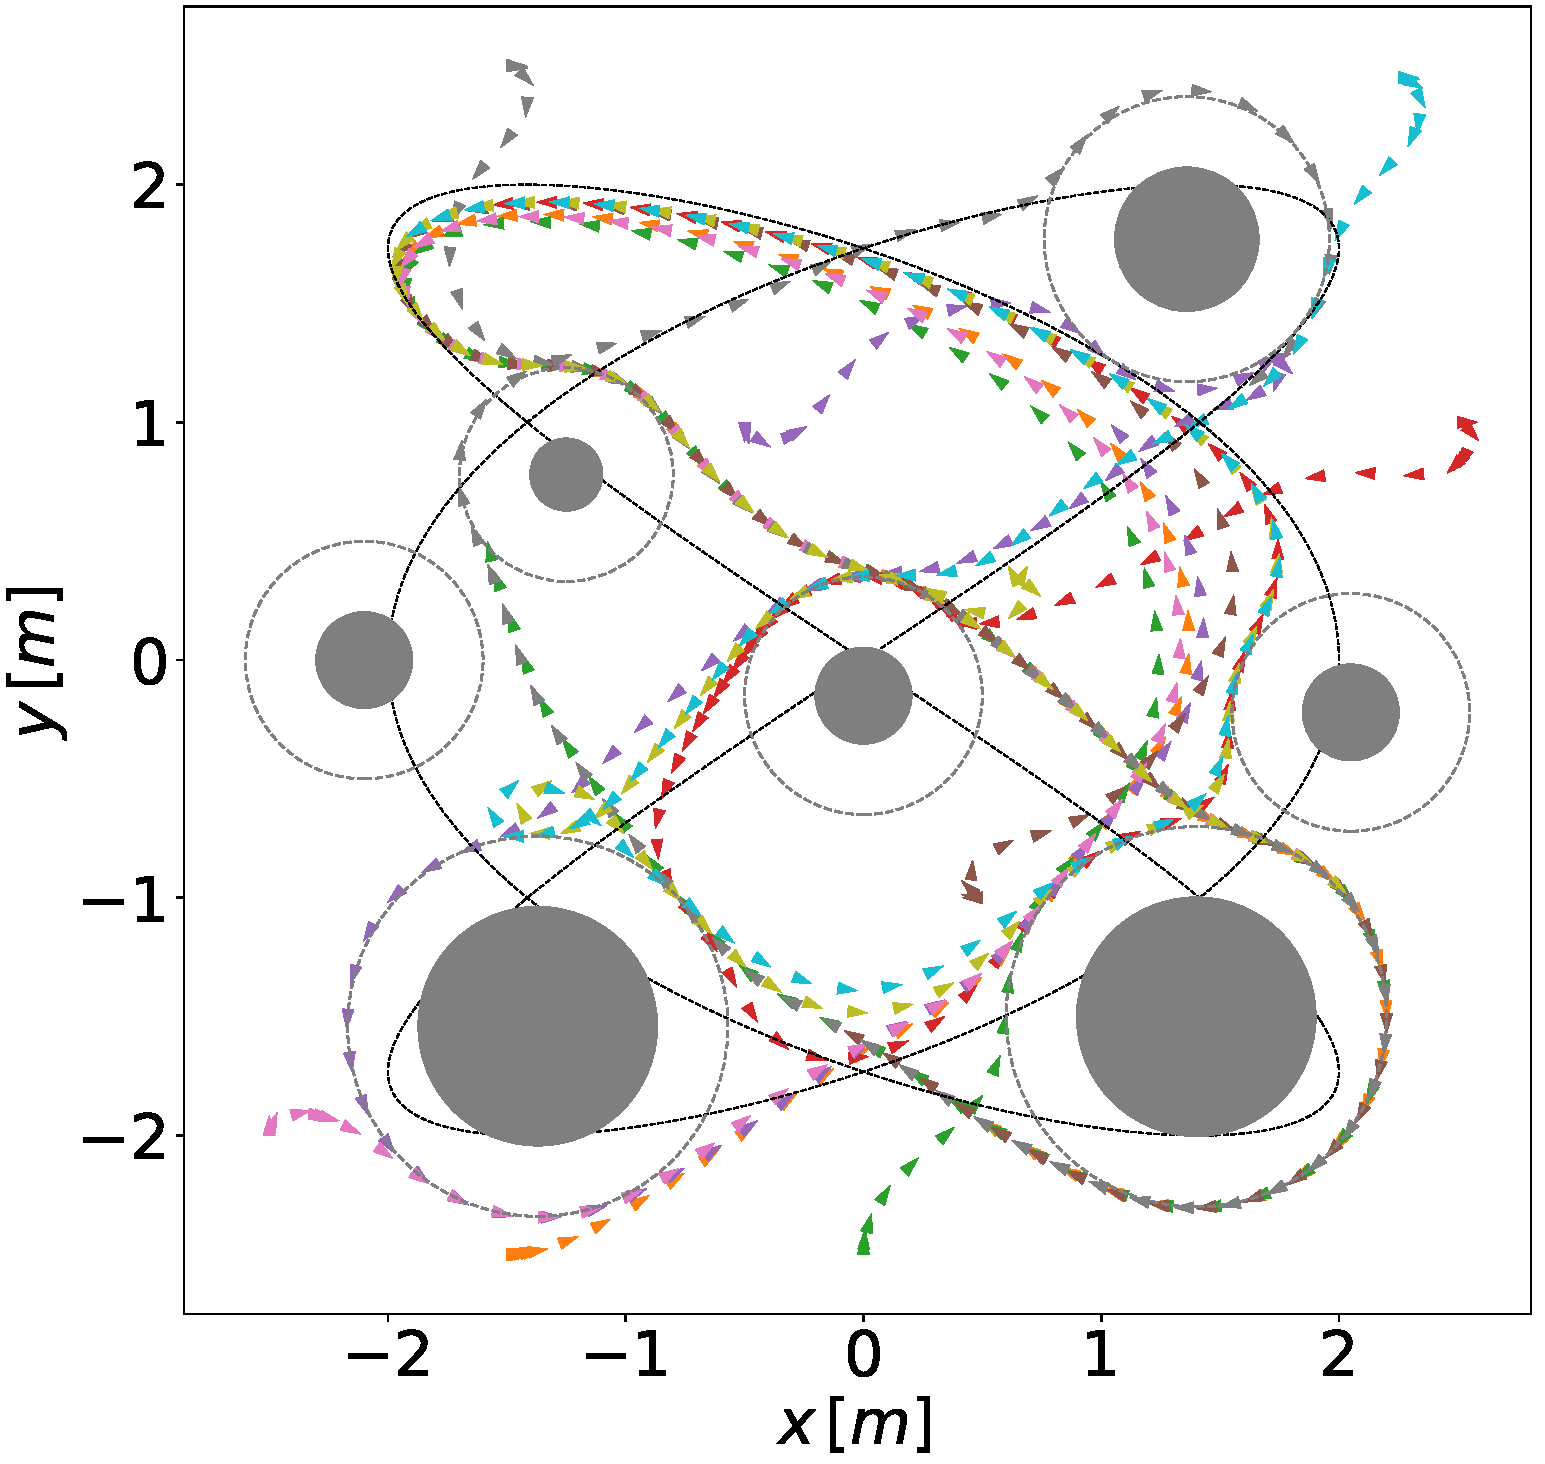
\includegraphics[width=0.49\linewidth]{Figures/Obstacle avoidance/Safe NMPC/Several_paths.pdf}}
  \end{subfigmatrix}
  \caption{Path tracking with safe one-stage real-time \acrshort{ocp} with solver $(1)$.}
  \label{fig:pathtrackingsafeocp}
\end{figure}

\begin{figure}
\centering
\begin{minipage}{.49\textwidth}
	\centering
  	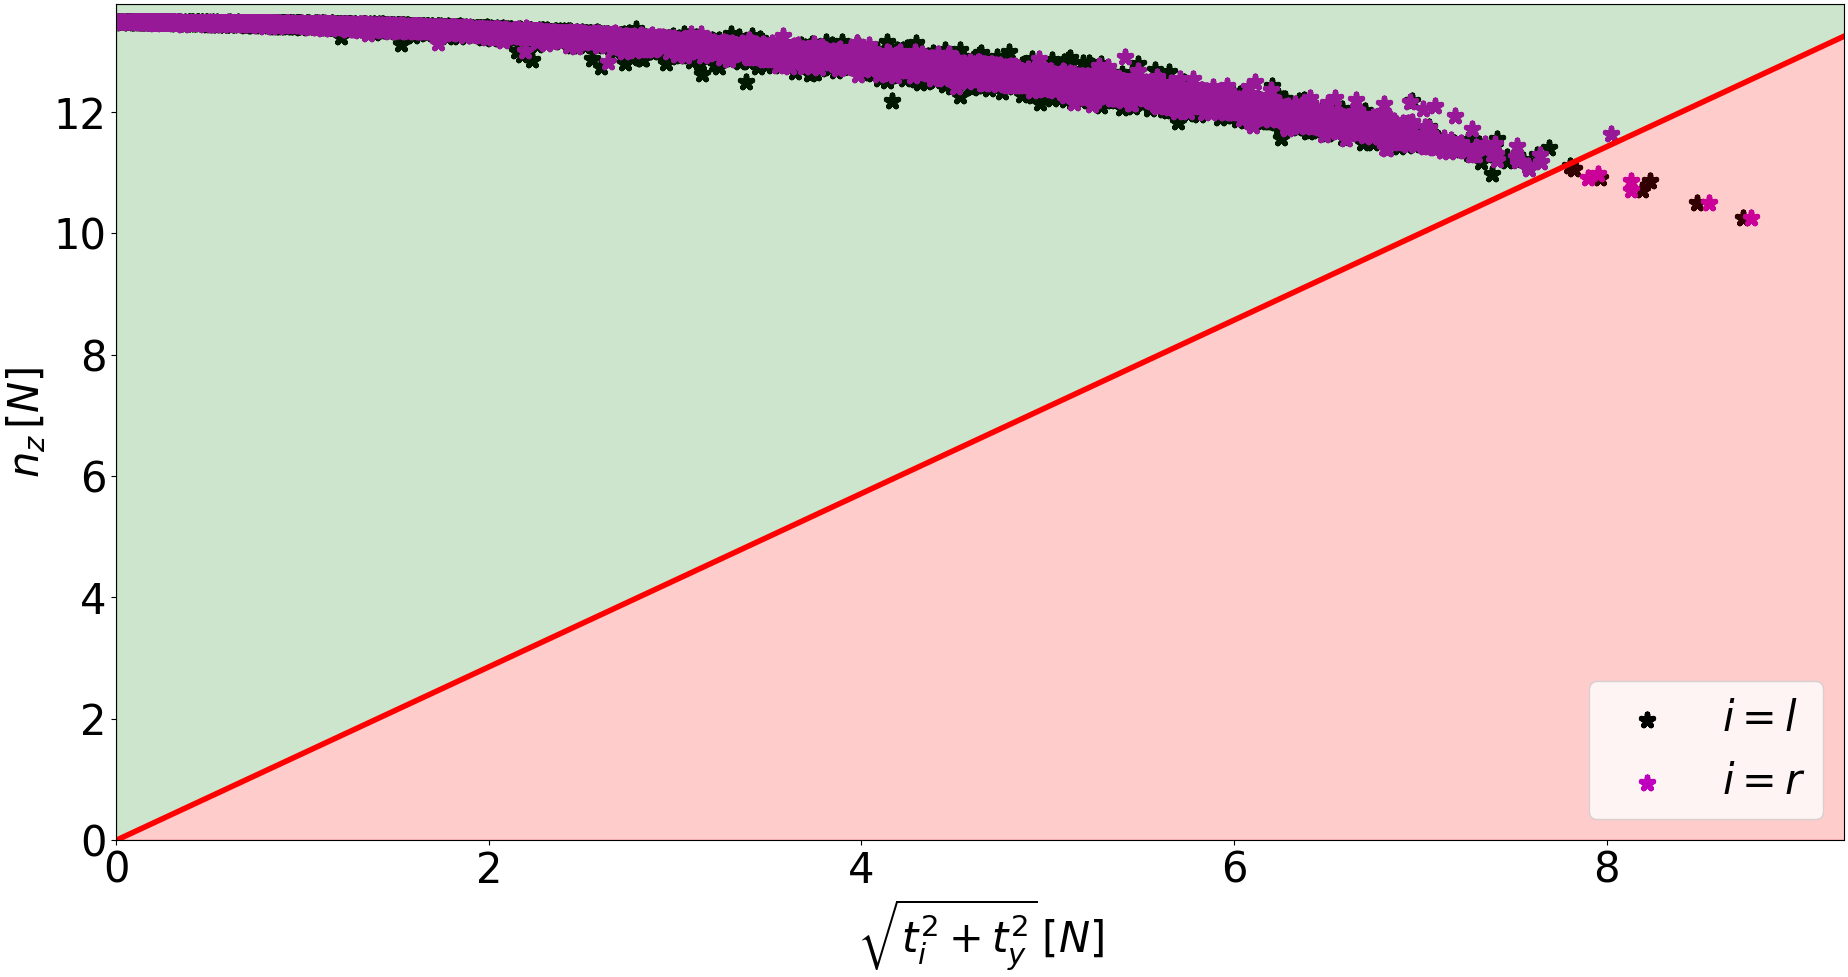
\includegraphics[width=0.95\linewidth]{Figures/Obstacle avoidance/Safe NMPC/forces_coulomb_cone.png}
  	\captionof{figure}{Traction forces within coulomb friction cone (solver $(1)$).}
  	\label{fig:frictionconesolver1}
\end{minipage}
\begin{minipage}{.49\textwidth}
	\centering  
  	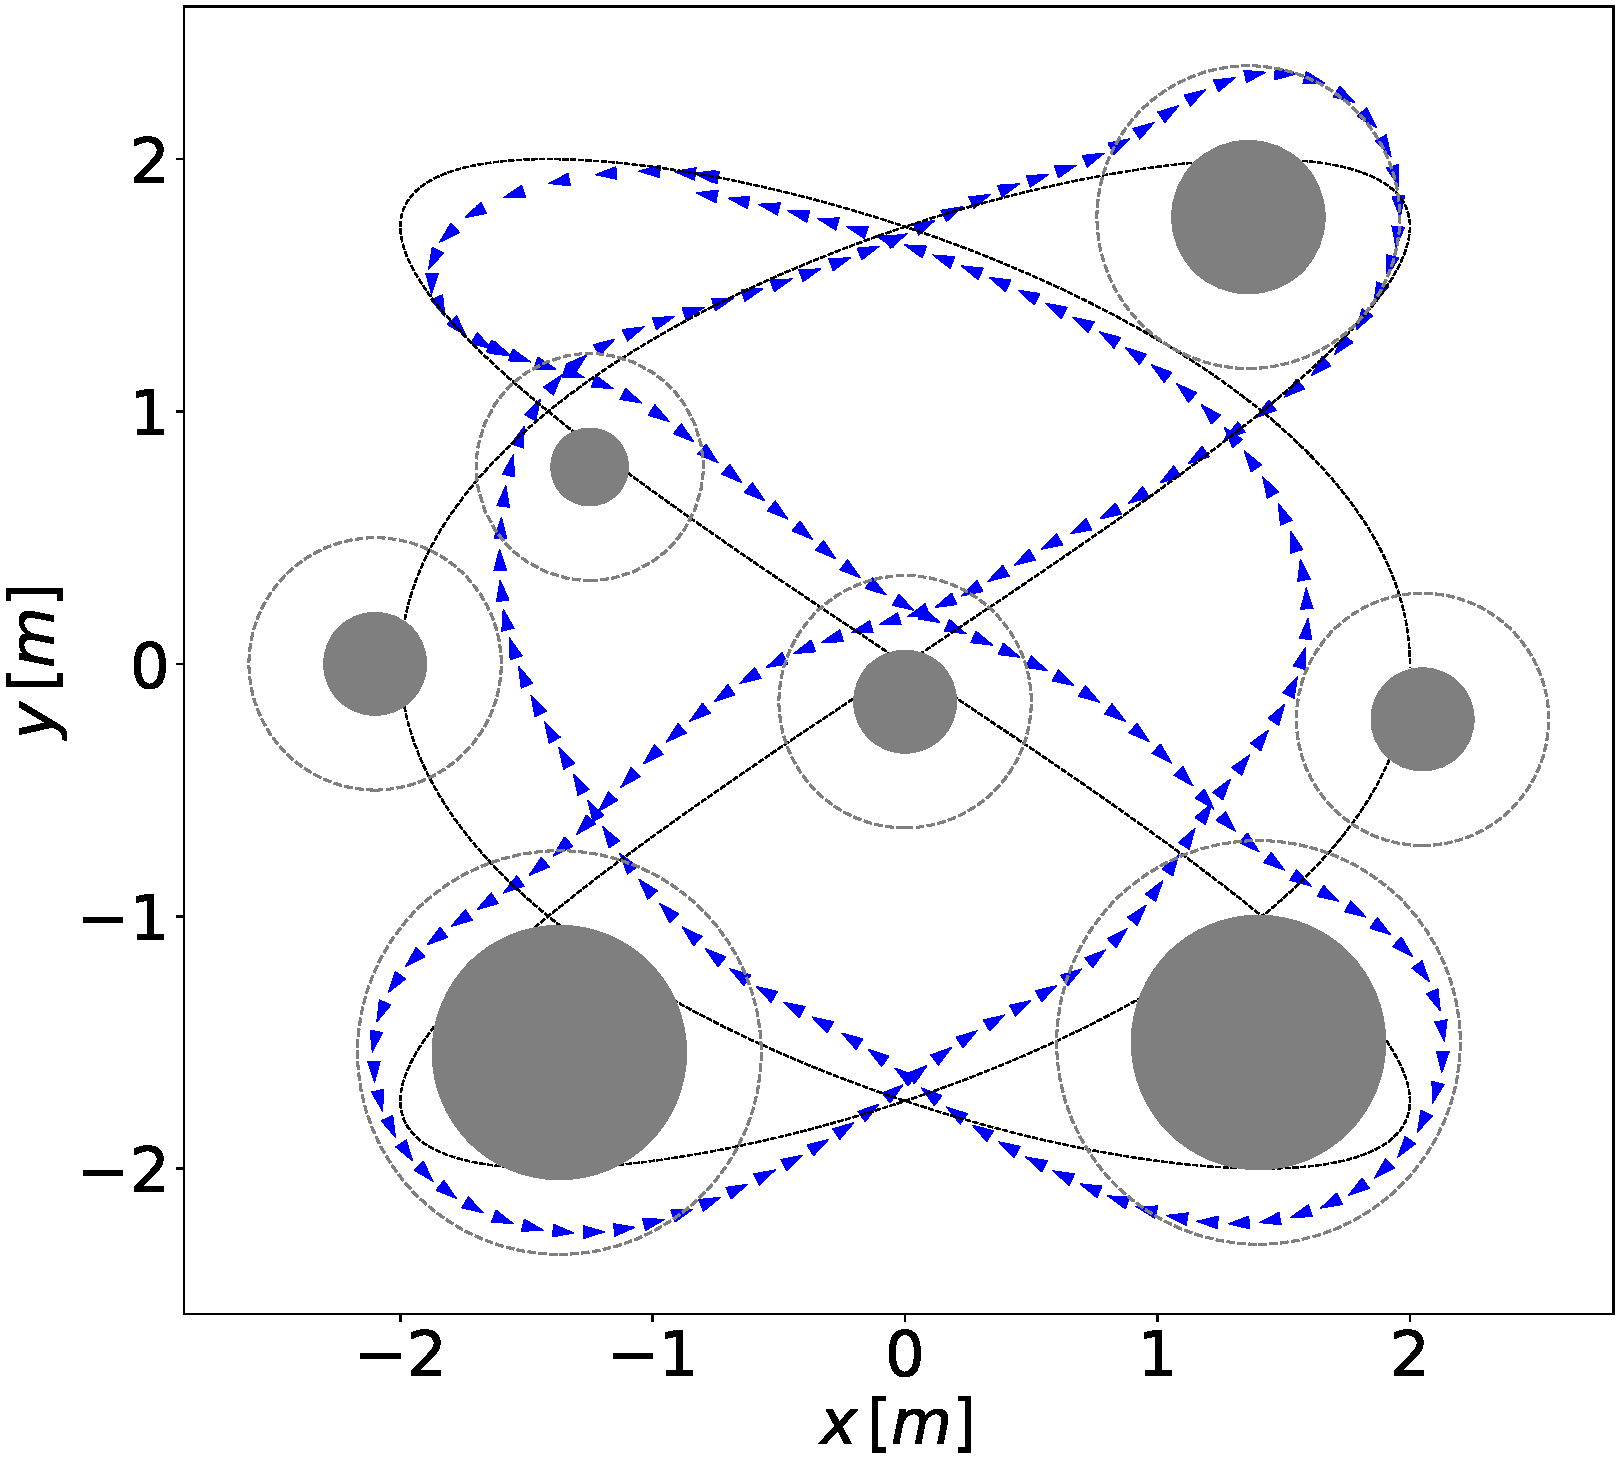
\includegraphics[width=0.95\linewidth]{Figures/Obstacle avoidance/Safe NMPC/tour_part1_solver_2.pdf}
  	\captionof{figure}{Reference tour with solver $(2)$.}
  	\label{fig:reftoursolver2}
\end{minipage}
\end{figure}

\subsubsection*{Slacks behaviour}

Slacks are activated  when the mobile robot enters $\overline{\SafeSpace}$. Figure \ref{fig:reftourperformancesolver1safeocp} clearly shows that. The zoomed in squares focus on points of the path where the maximum slack among the horizon of slacks is very high. The fact that the mobile robot moves into $\overline{\SafeSpace}$ forces the solver to activate the slacks, in order to avoid solver failure. This is once again reassured by the top picture of the left figure of \ref{fig:reftourperformancesolver1safeocp}, where the clearance of the mobile robot is plotted against the maximum slack. It is seen that slacks are activated when the clearance is minimal. Figure \ref{fig:maxslackpathref} only shows one tour of the reference, whereas the data of figure \ref{fig:reftourperformancesolver1safeocp} depicts data of three tours.

Along the whole reference tour, the minimum recorded clearance was $0.287\,m$ (solver $(1)$). In the case of solver $(2)$, the minimum recorded clearance was $0.12\,m$. This shows that solver $(1)$ safeguards the mobile robot's safety, whereas solver $(2)$ compromises it.

The solver optimal cost is rarely small as the the pose horizon cannot eliminate the pose error due to the spatial restrictions introduced by the presence of obstacles. The loop time is often below the sampling time. $10$ timeouts were recorded in more than $20000$ simulation iterations.

\begin{figure}
	\centering
	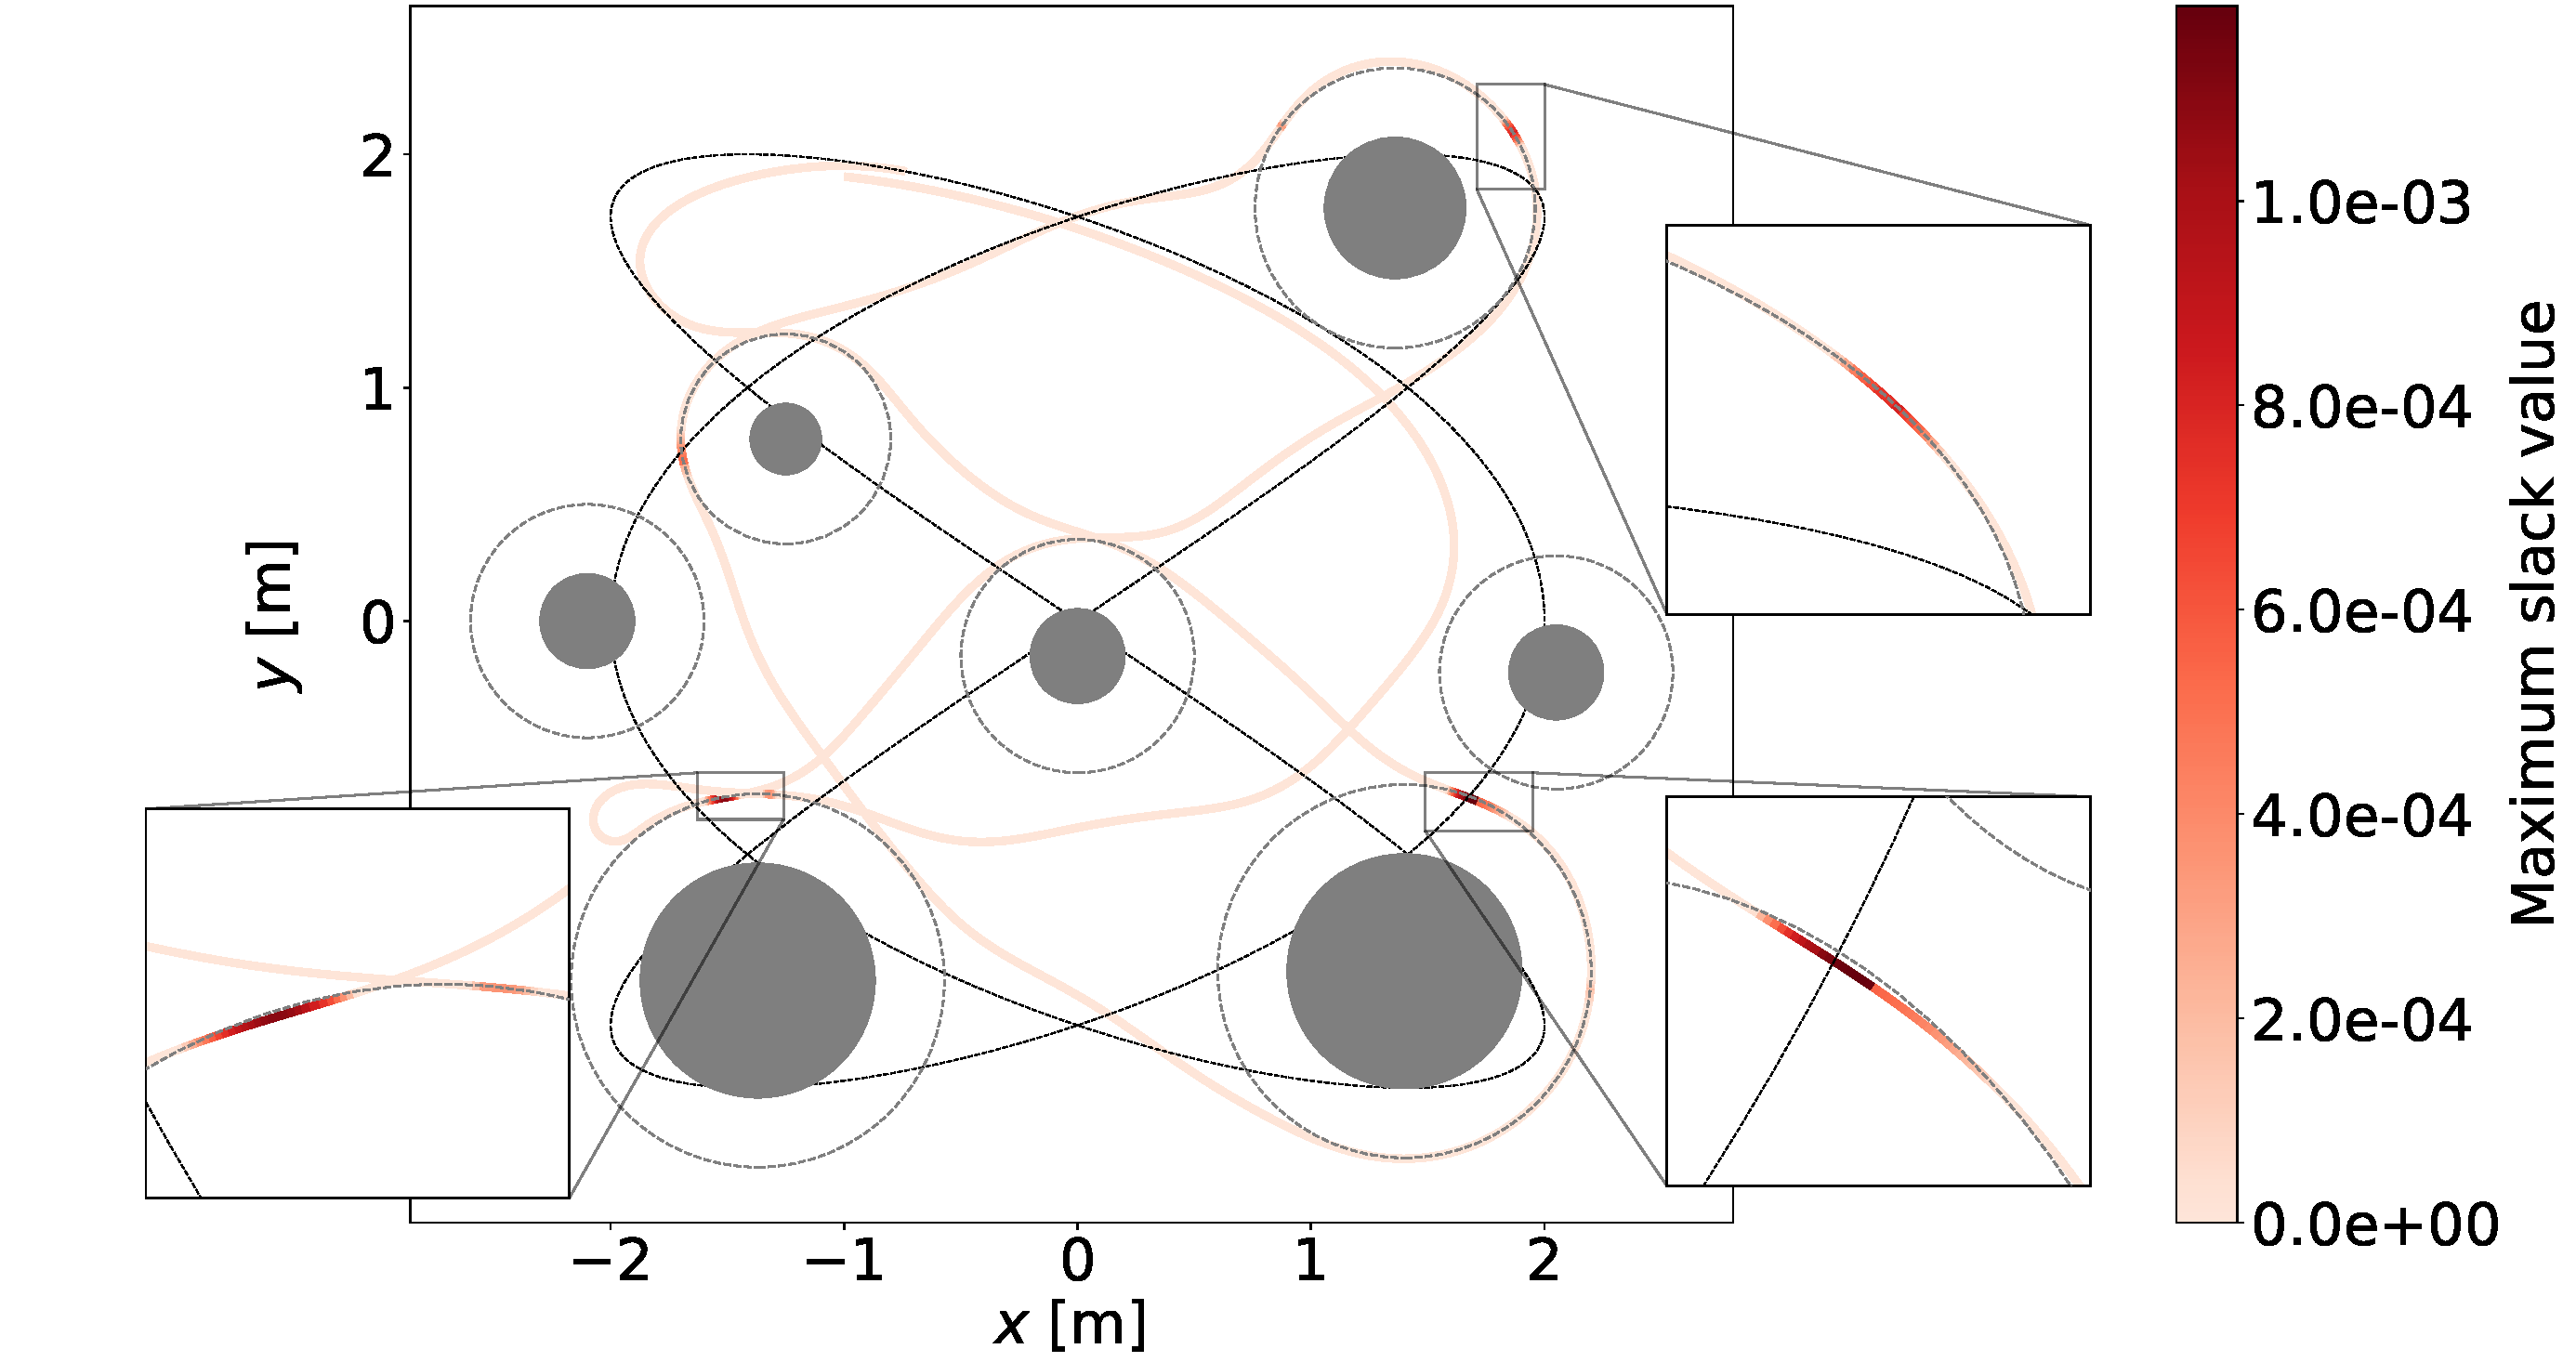
\includegraphics[width=0.98\linewidth]{Figures/Obstacle avoidance/Safe NMPC/slacks_path_tracking_solver_1_tour_1.pdf}
	\caption{Maximum slack among slacks horizon at each simulation iteration.}
	\label{fig:maxslackpathref}
\end{figure}

\begin{figure}[!htb]
  \begin{subfigmatrix}{2}
    \subfigure[Maximum slack vs clearance (top). Optimal cost (middle). Loop time (bottom).]{
    	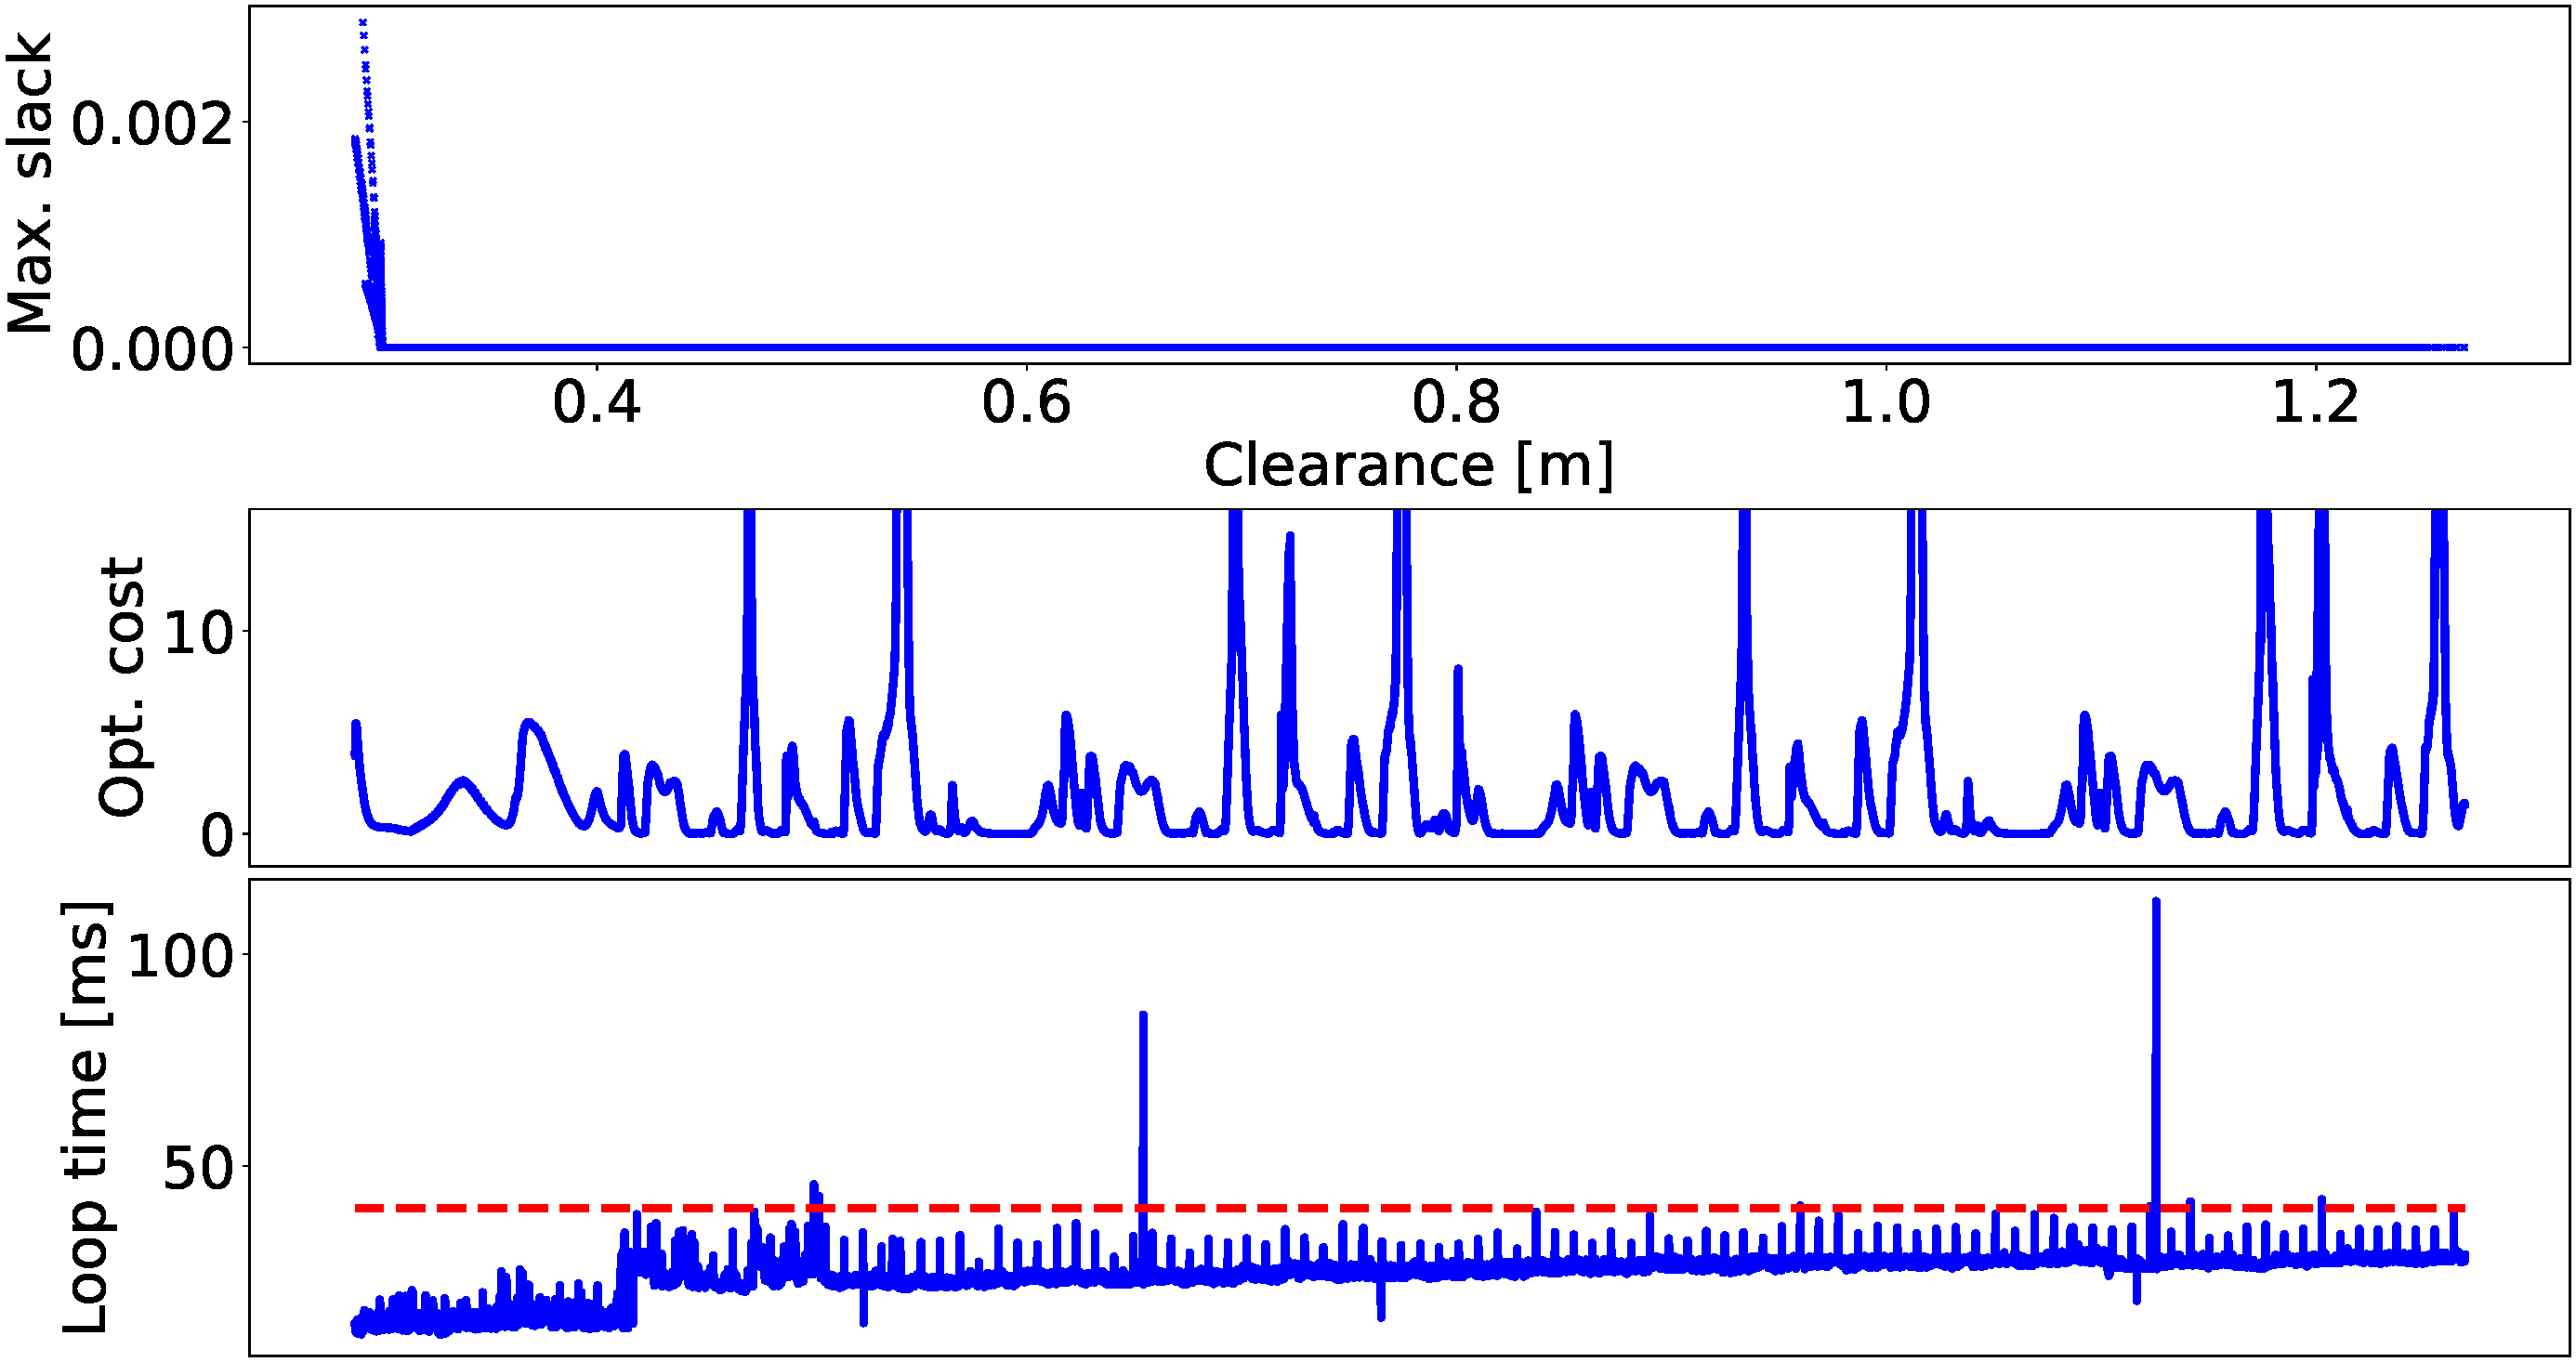
\includegraphics[width=0.49\linewidth]{Figures/Obstacle avoidance/Safe NMPC/solver_1_tour_1_specs.pdf}}
    \subfigure[Linear and angular velocities (top). Force rates (bottom).]{
    	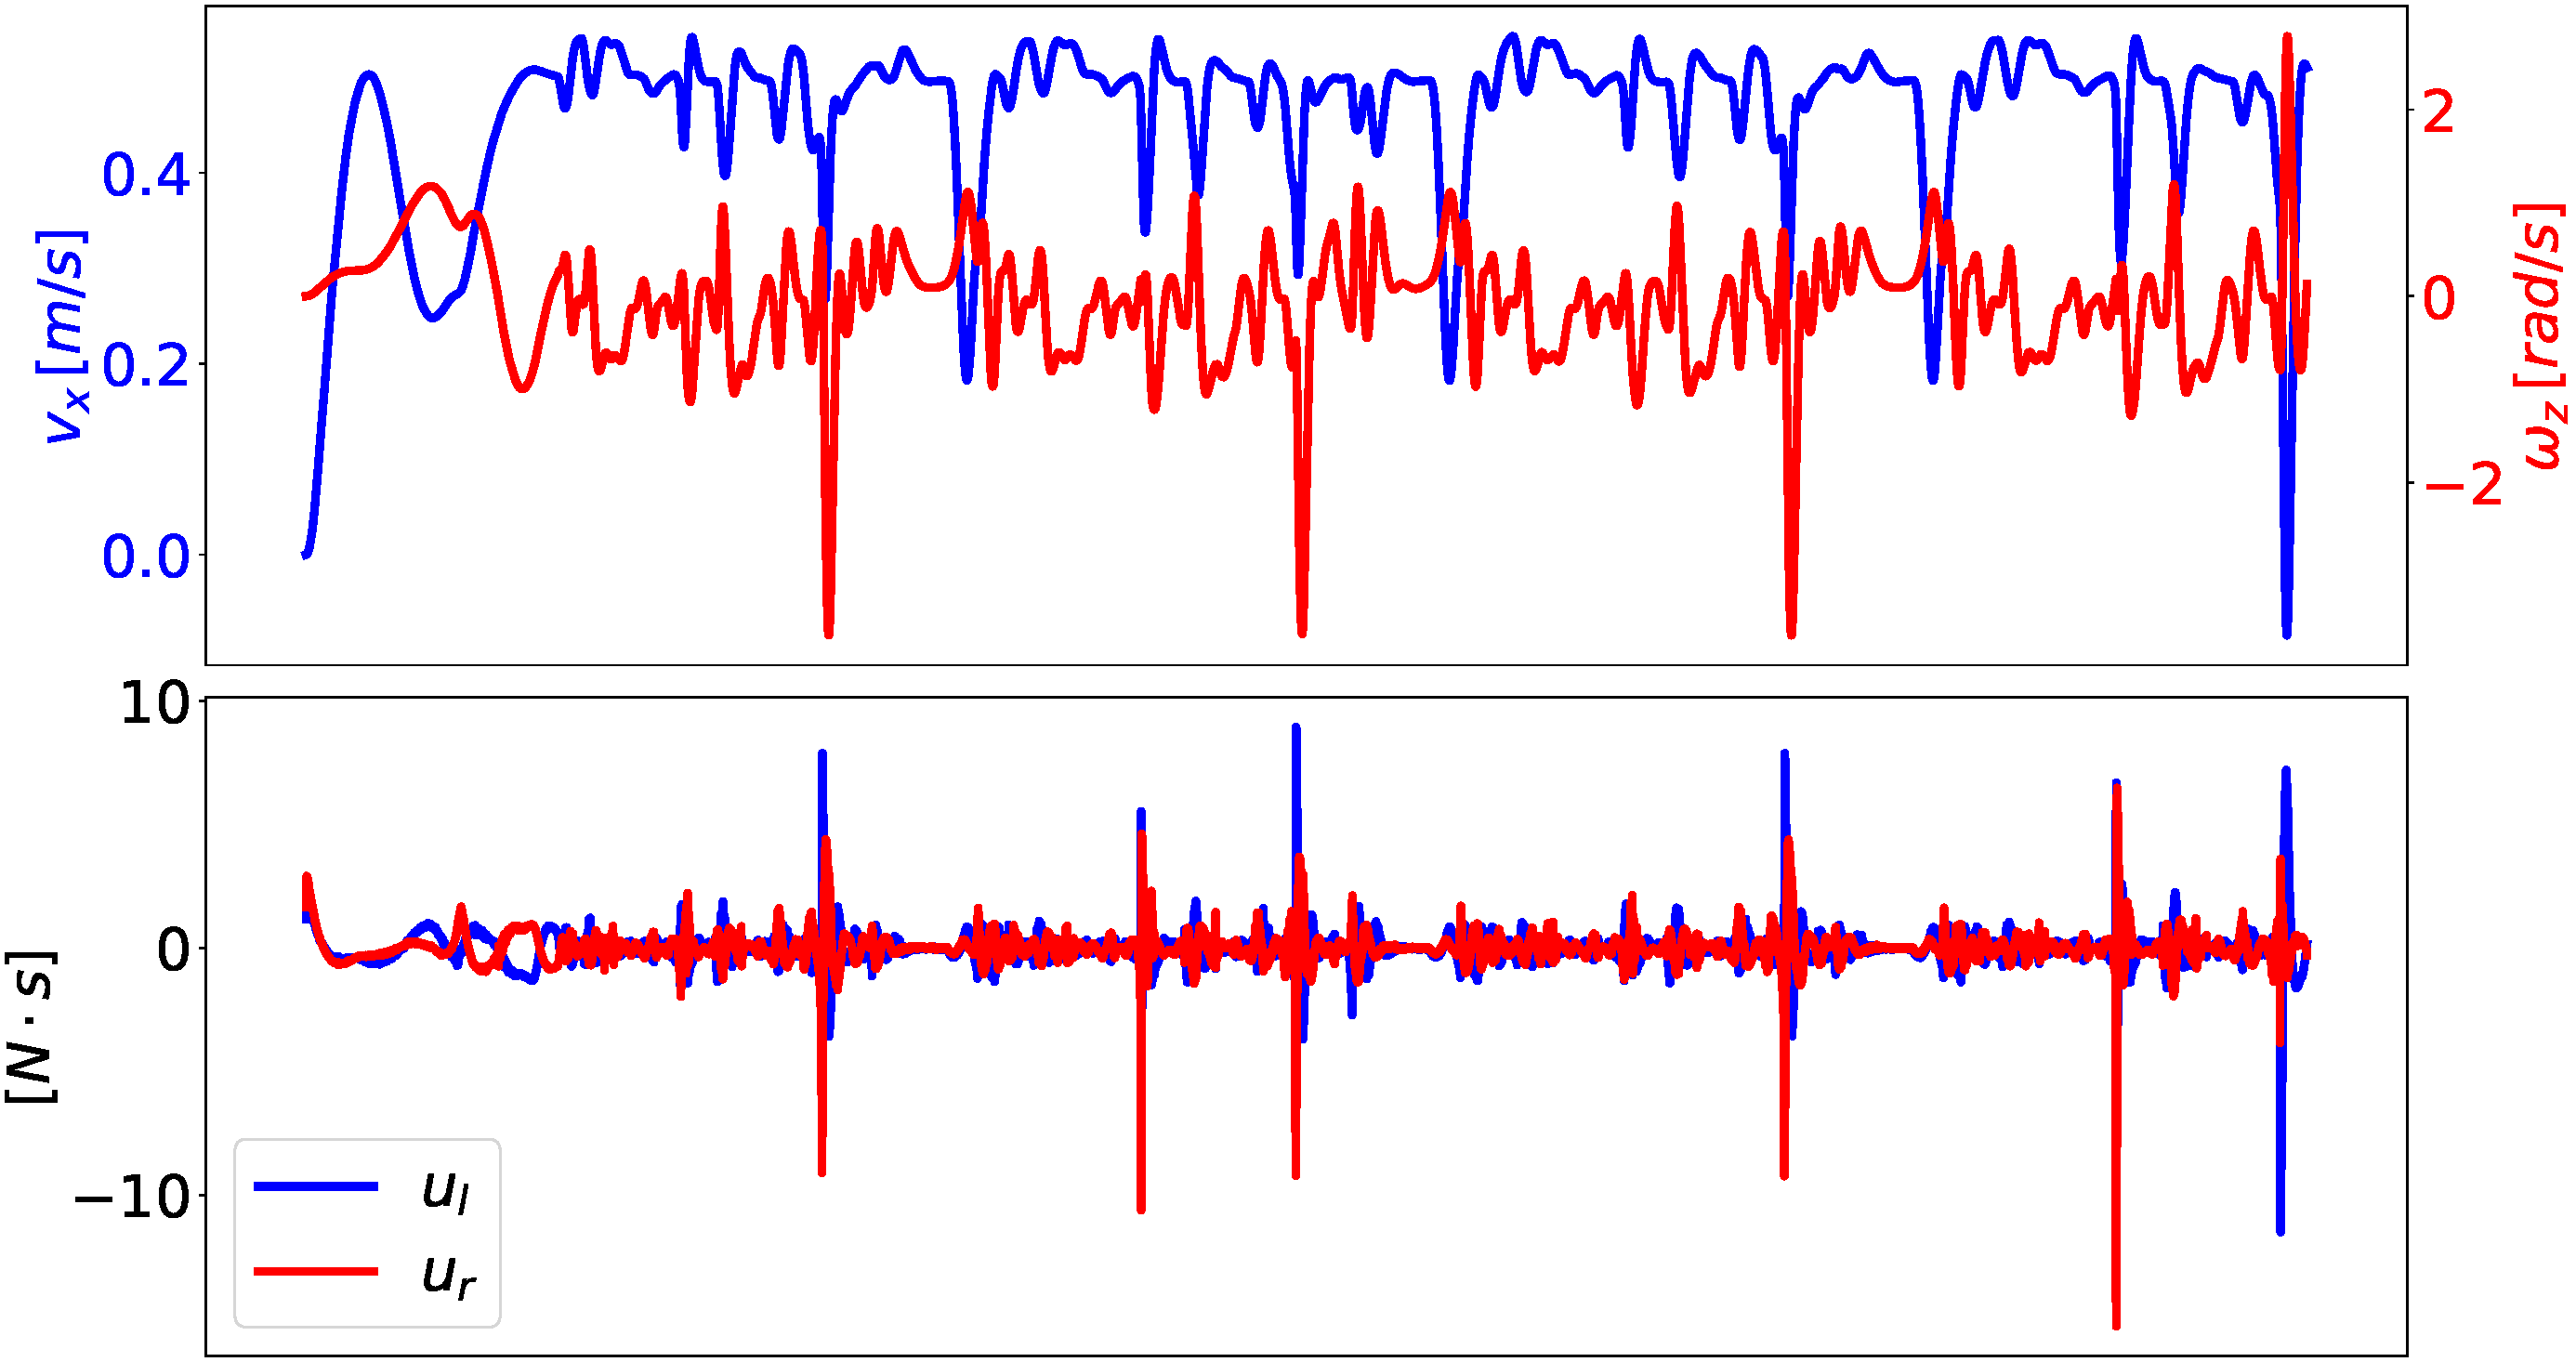
\includegraphics[width=0.49\linewidth]{Figures/Obstacle avoidance/Safe NMPC/vel_forces_rate_solver_1_tour_1.pdf}}
  \end{subfigmatrix}
  \caption{Reference tour performance plus velocities and force rates curves with solver $(1)$.}
  \label{fig:reftourperformancesolver1safeocp}
\end{figure}

The linear velocity reaches a maximum of $0.5\,m/s$ which is within a reasonably safe linear velocity range. The rate of forces curve presents an up and down around 0 with non-negligible rates that reach higher values sometimes. As the weight of the controls is $1.0$, the rate of forces horizon is an important contributor to the optimal cost value. 

\subsubsection*{Safe balls evolution}

Before the chapter's end, it is relevant to show the safe balls evolution along the horizon on critical points of the simulation. Figure \ref{fig:safeballsexamplessolver1} presents the reference position horizon, the optimal position horizon and the safe balls that were computed with respect to the previous optimal position horizon. As the next optimal position horizon is meant to be close to the previous one, the current set of safe balls very closely express the positional constraint of the next solution.

\begin{figure}[!htb]
  \begin{subfigmatrix}{6}
    \subfigure[Far away from closest obstacle.]{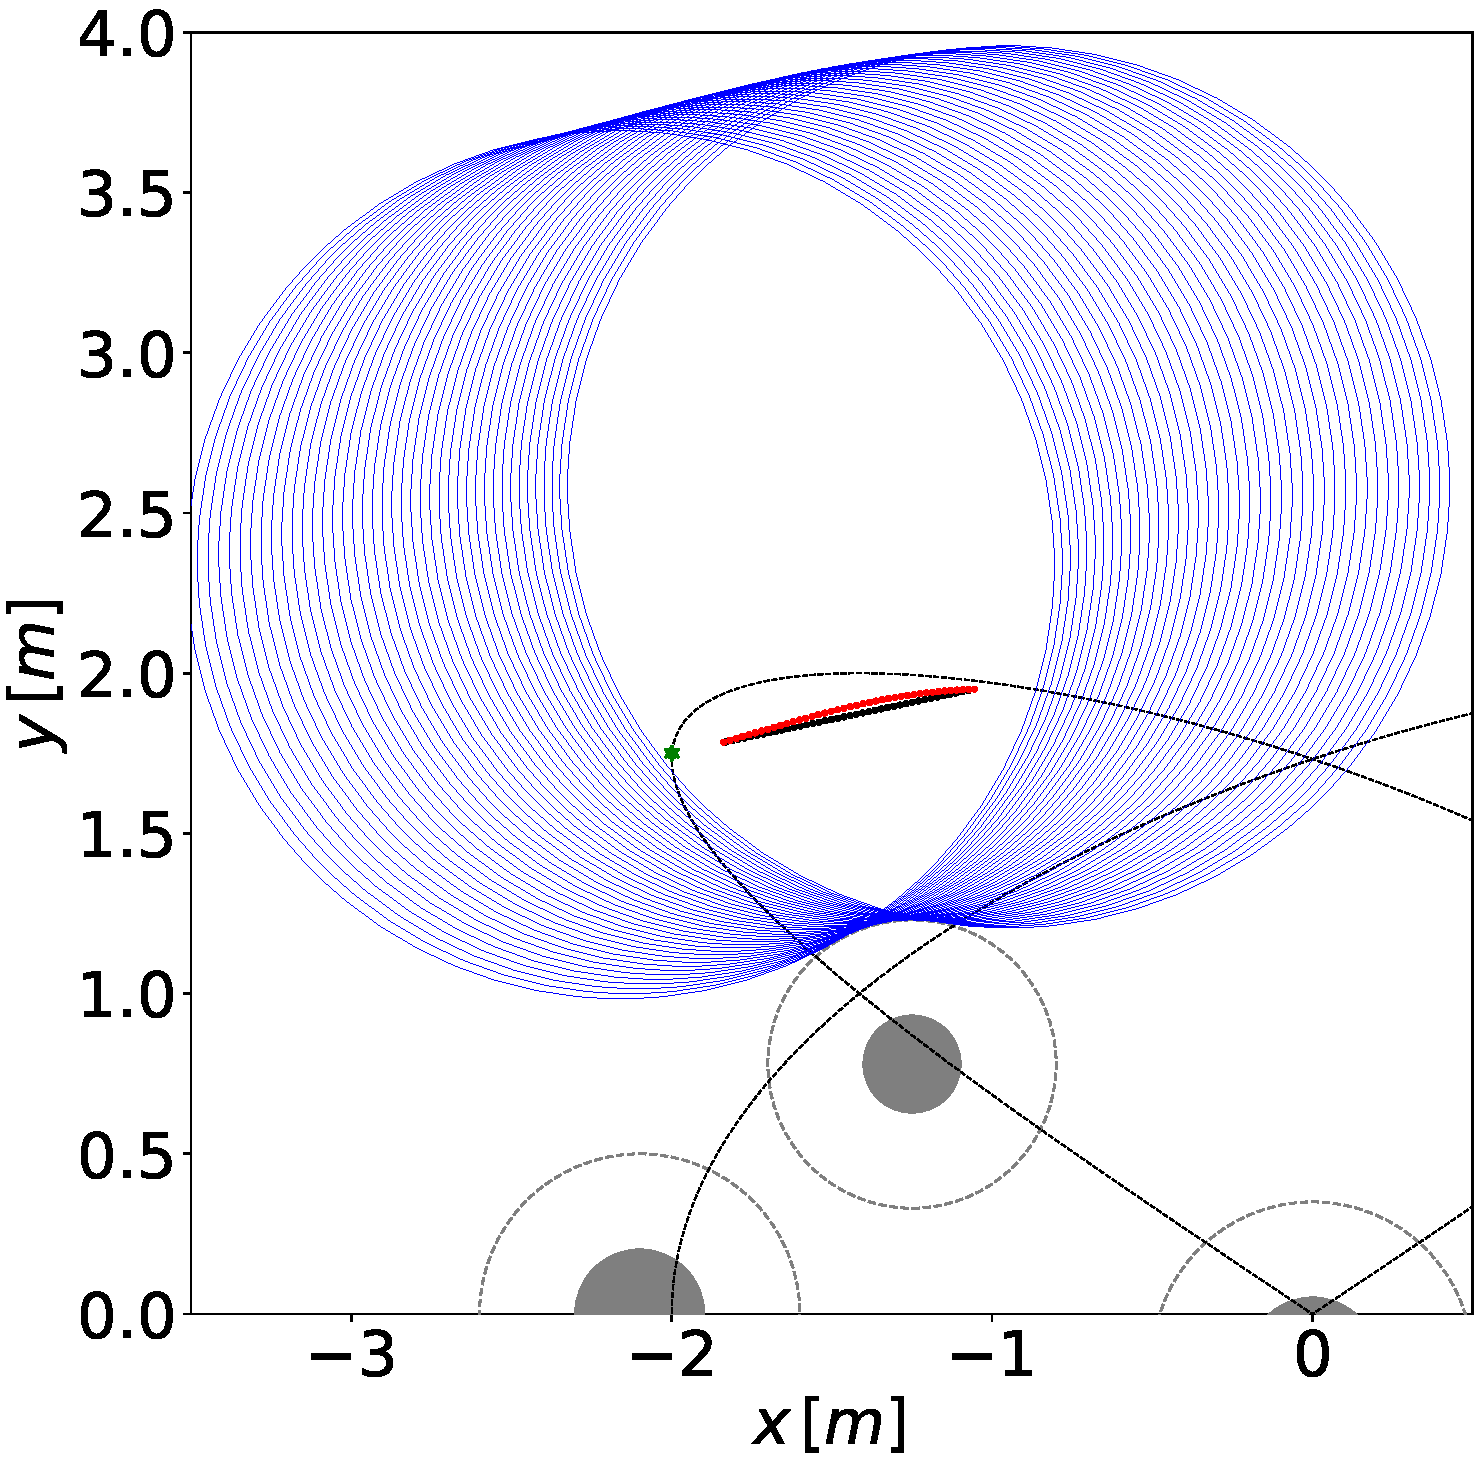
\includegraphics[width=0.32\linewidth]{Figures/Obstacle avoidance/Safe NMPC/example_ciao_circles_1.pdf}}
    \subfigure[Stuck while projected target does not move.]{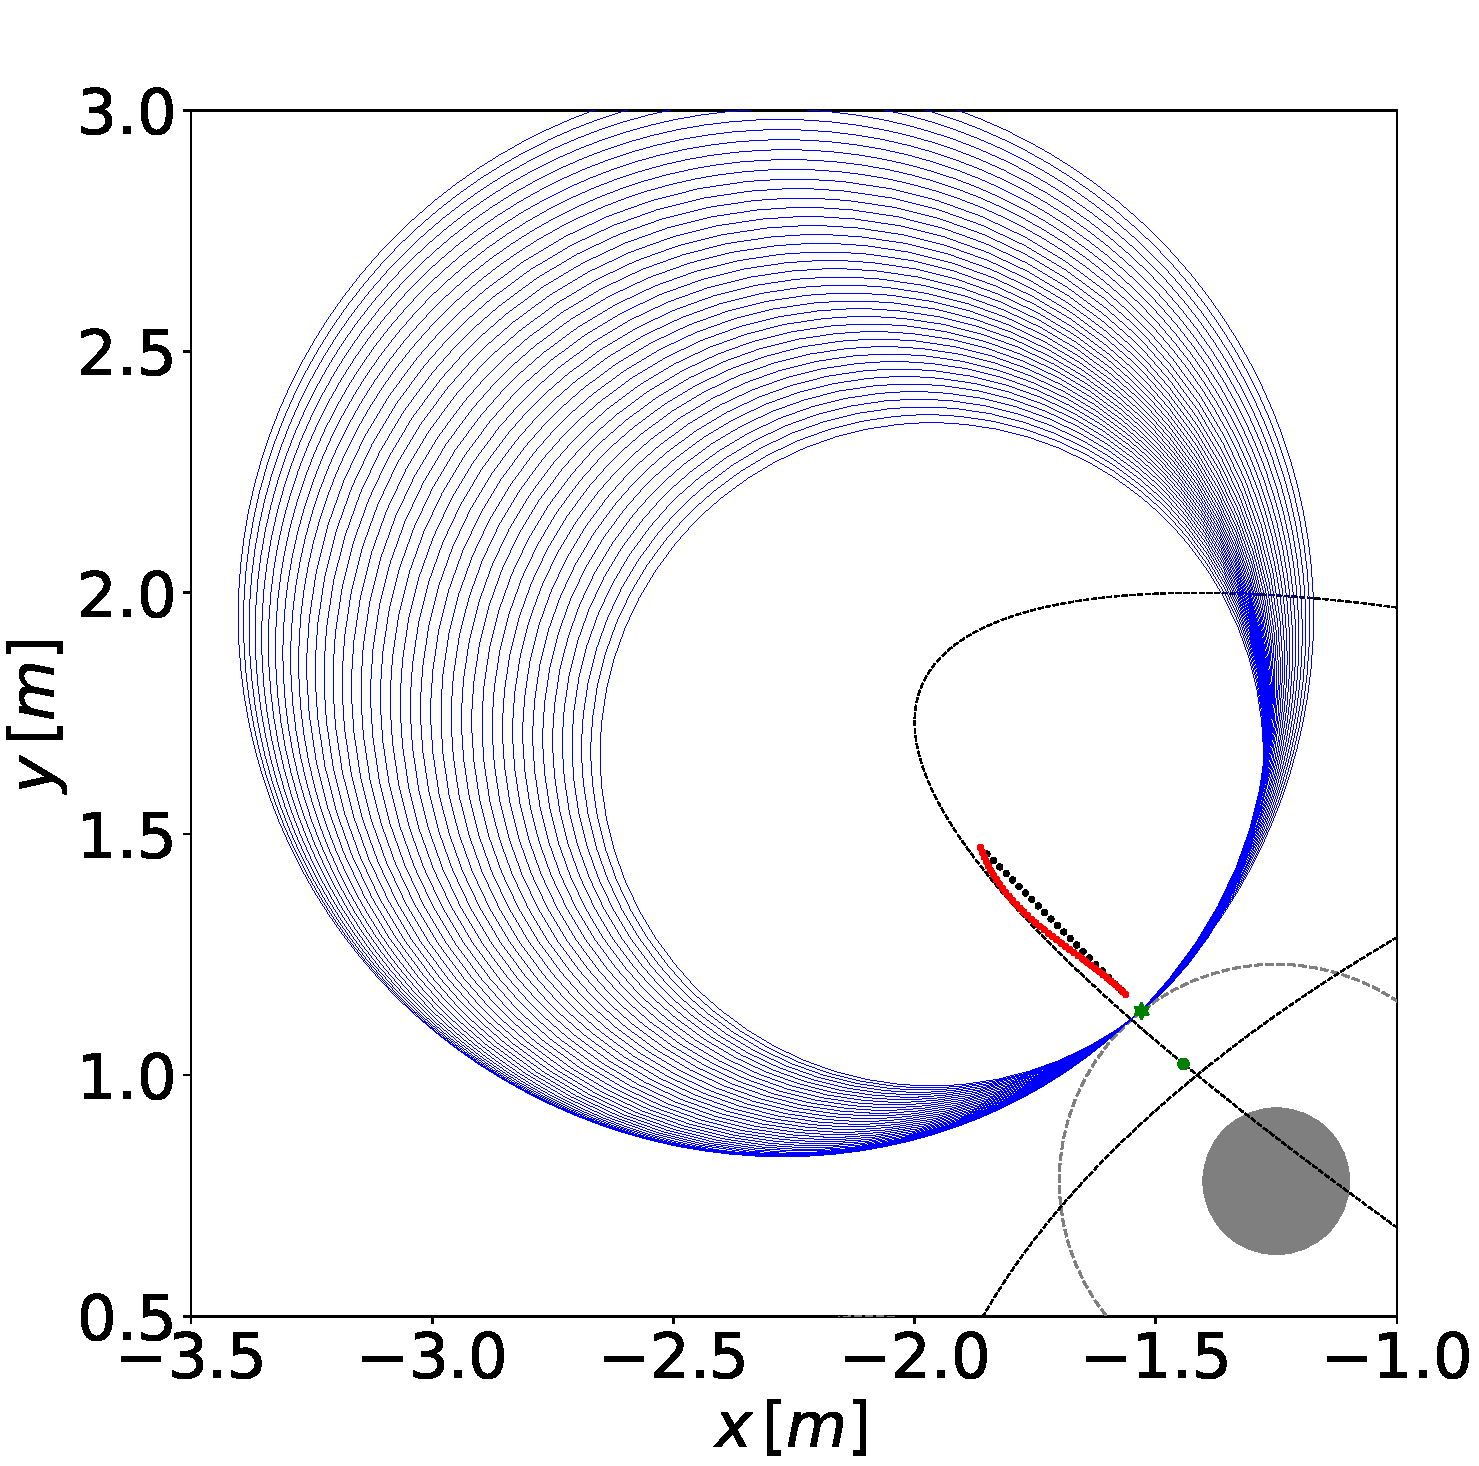
\includegraphics[width=0.32\linewidth]{Figures/Obstacle avoidance/Safe NMPC/example_ciao_circles_2.pdf}}
    \subfigure[Very narrow traversal between obstacles.]{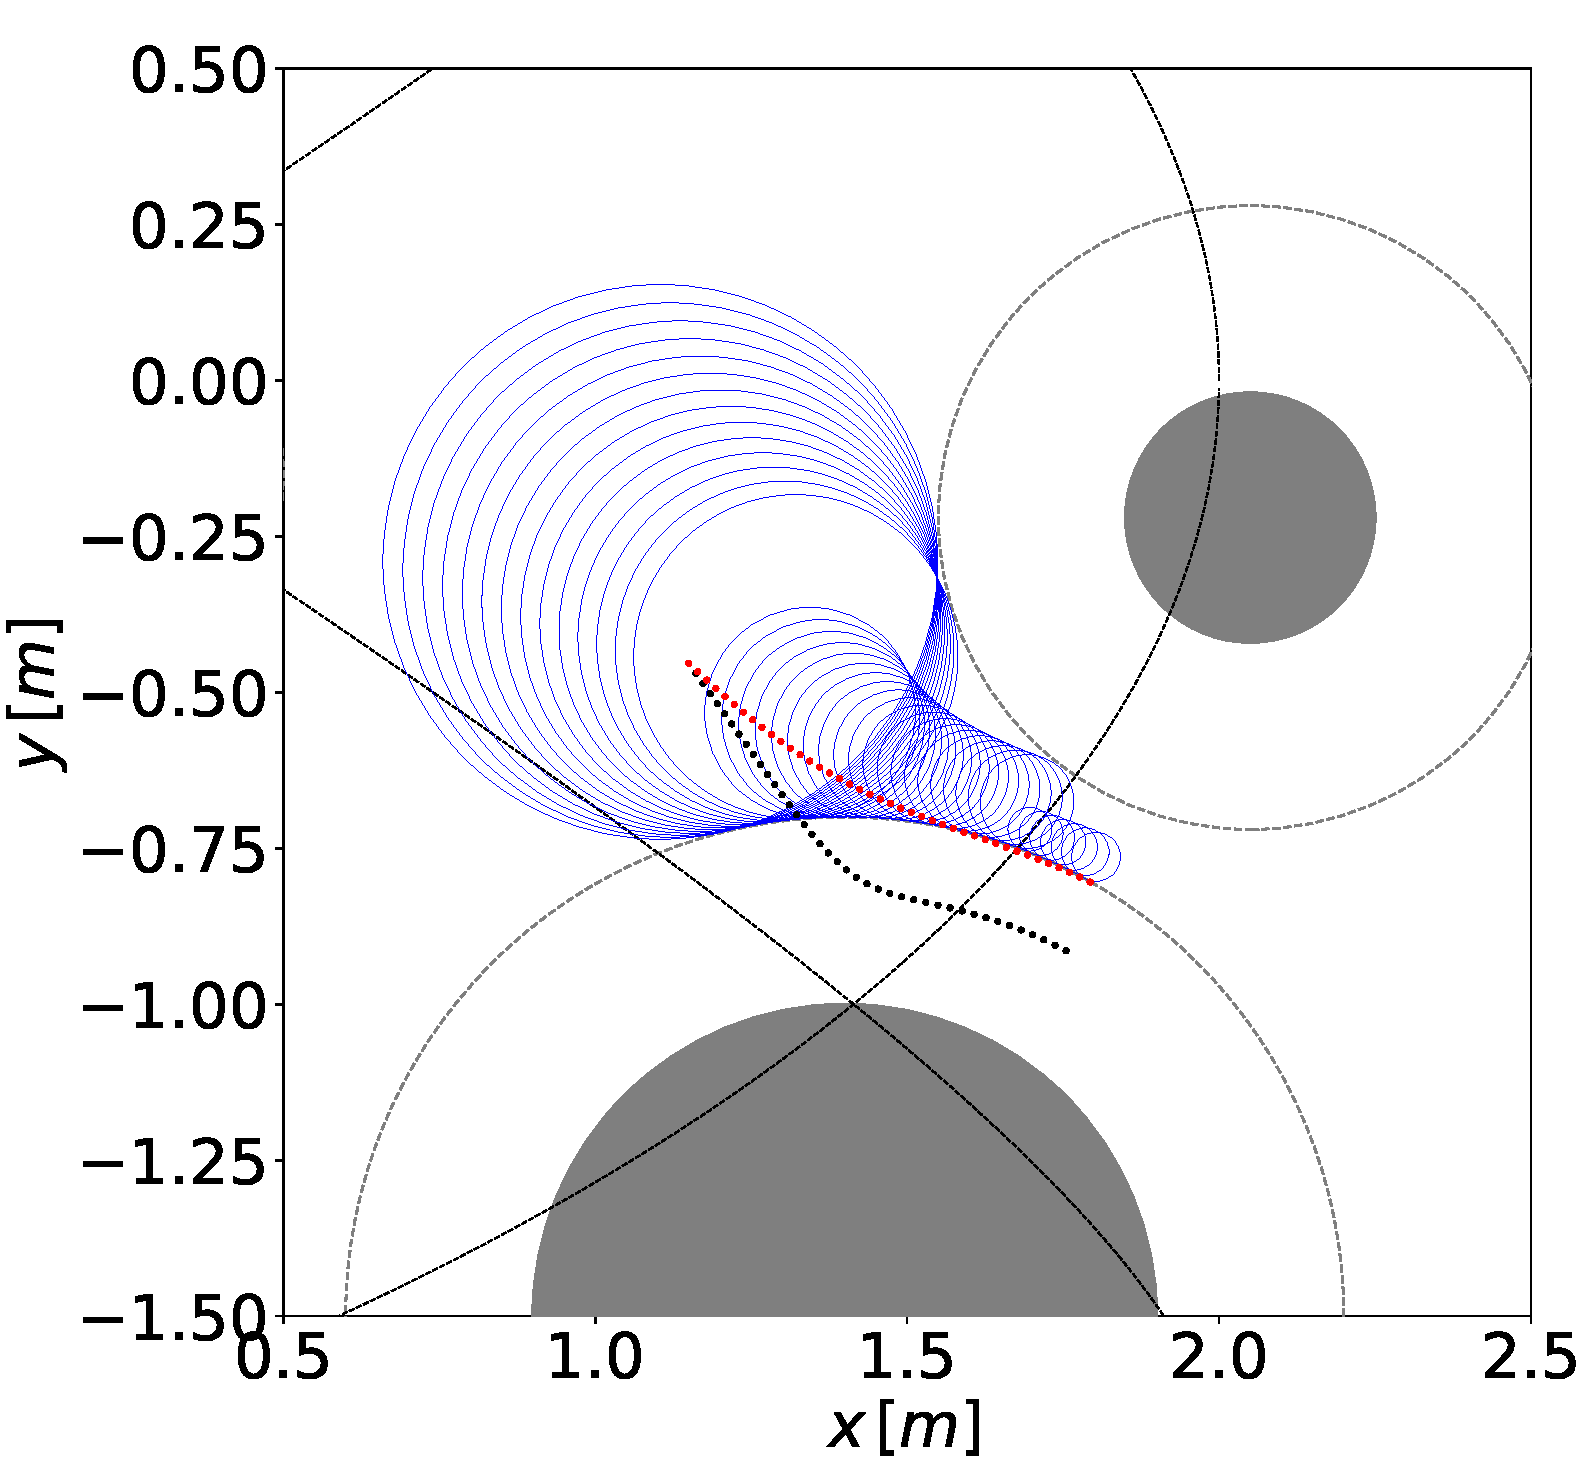
\includegraphics[width=0.32\linewidth]{Figures/Obstacle avoidance/Safe NMPC/example_ciao_circles_4.pdf}}
    \subfigure[Turn around.]{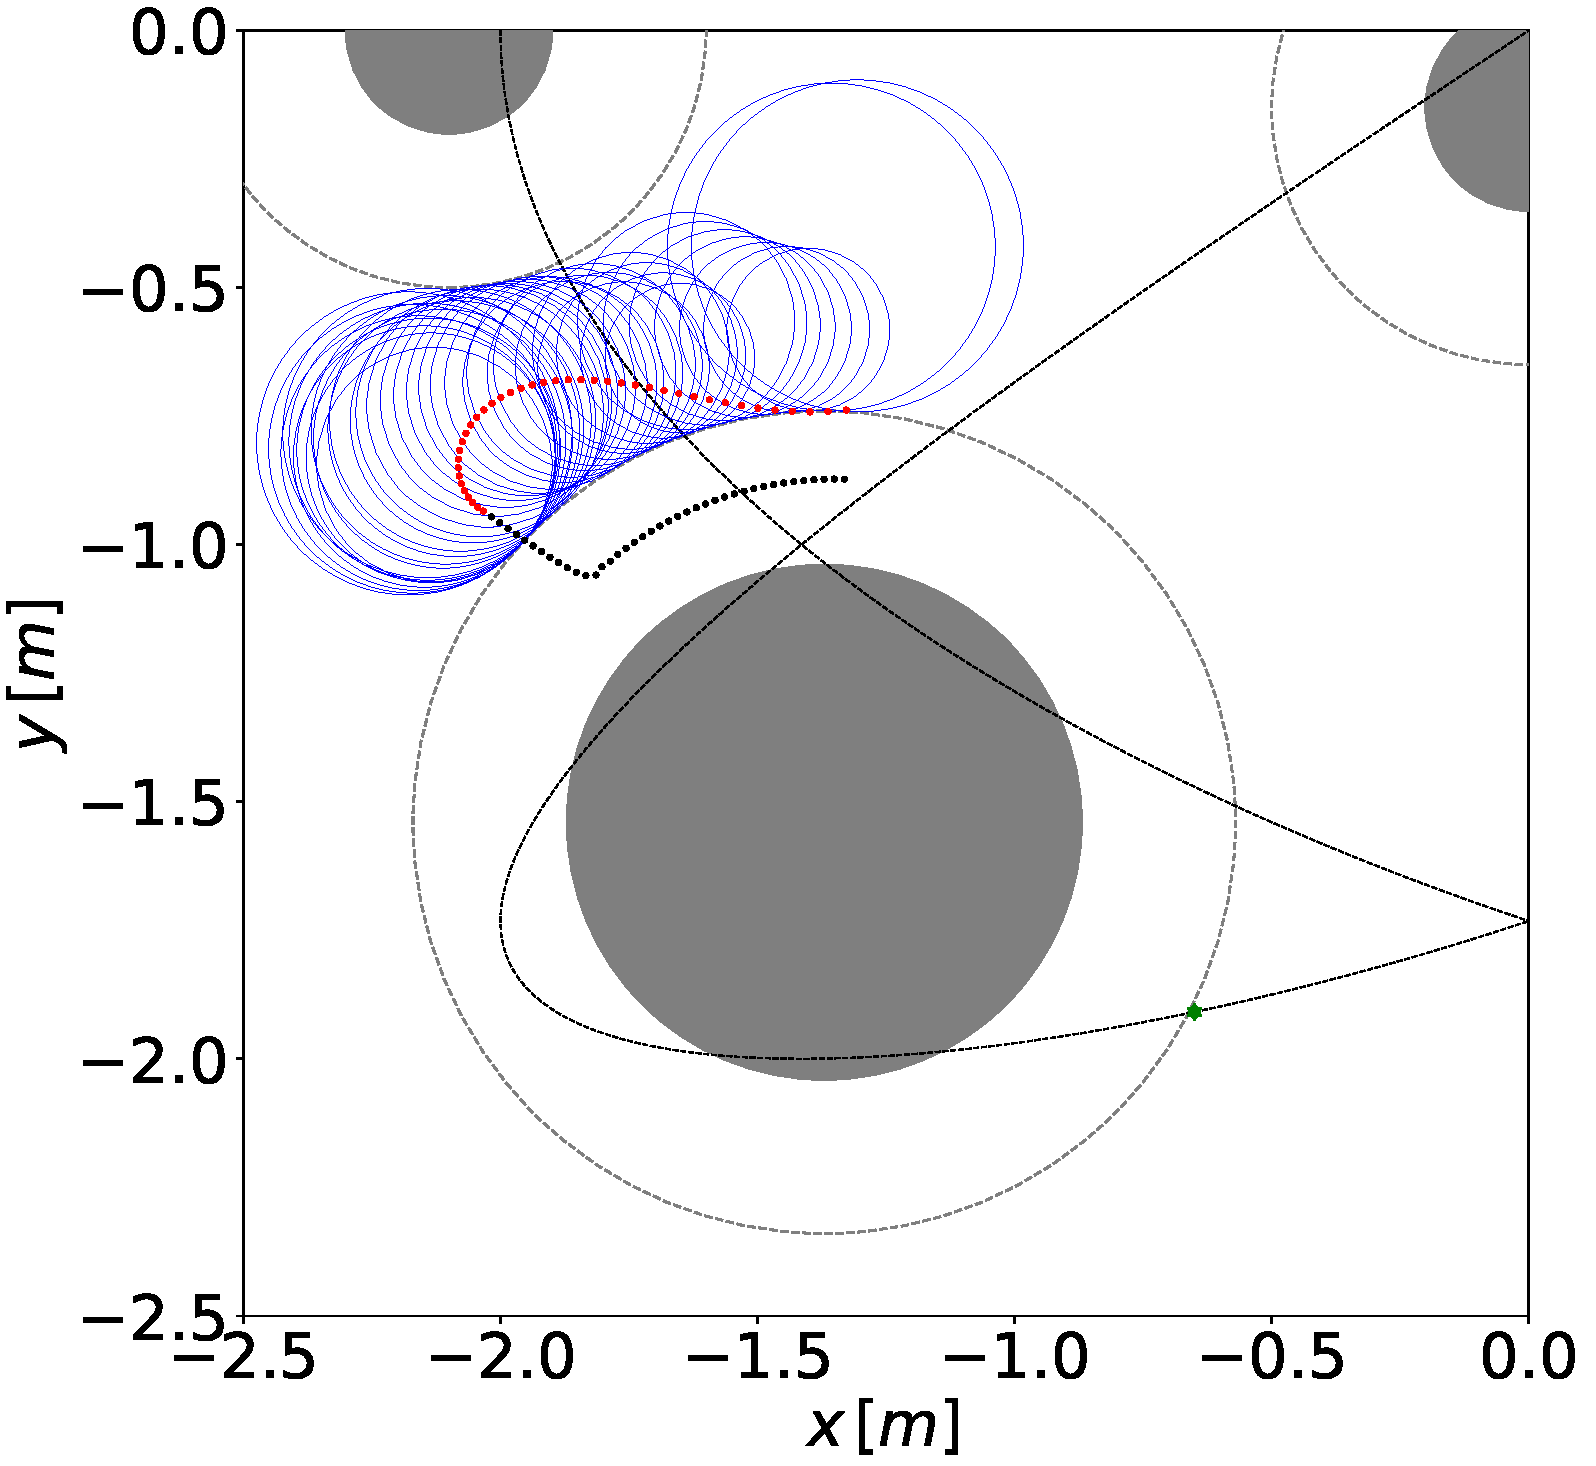
\includegraphics[width=0.32\linewidth]{Figures/Obstacle avoidance/Safe NMPC/example_ciao_circles_9.pdf}}
    \subfigure[High cost event.]{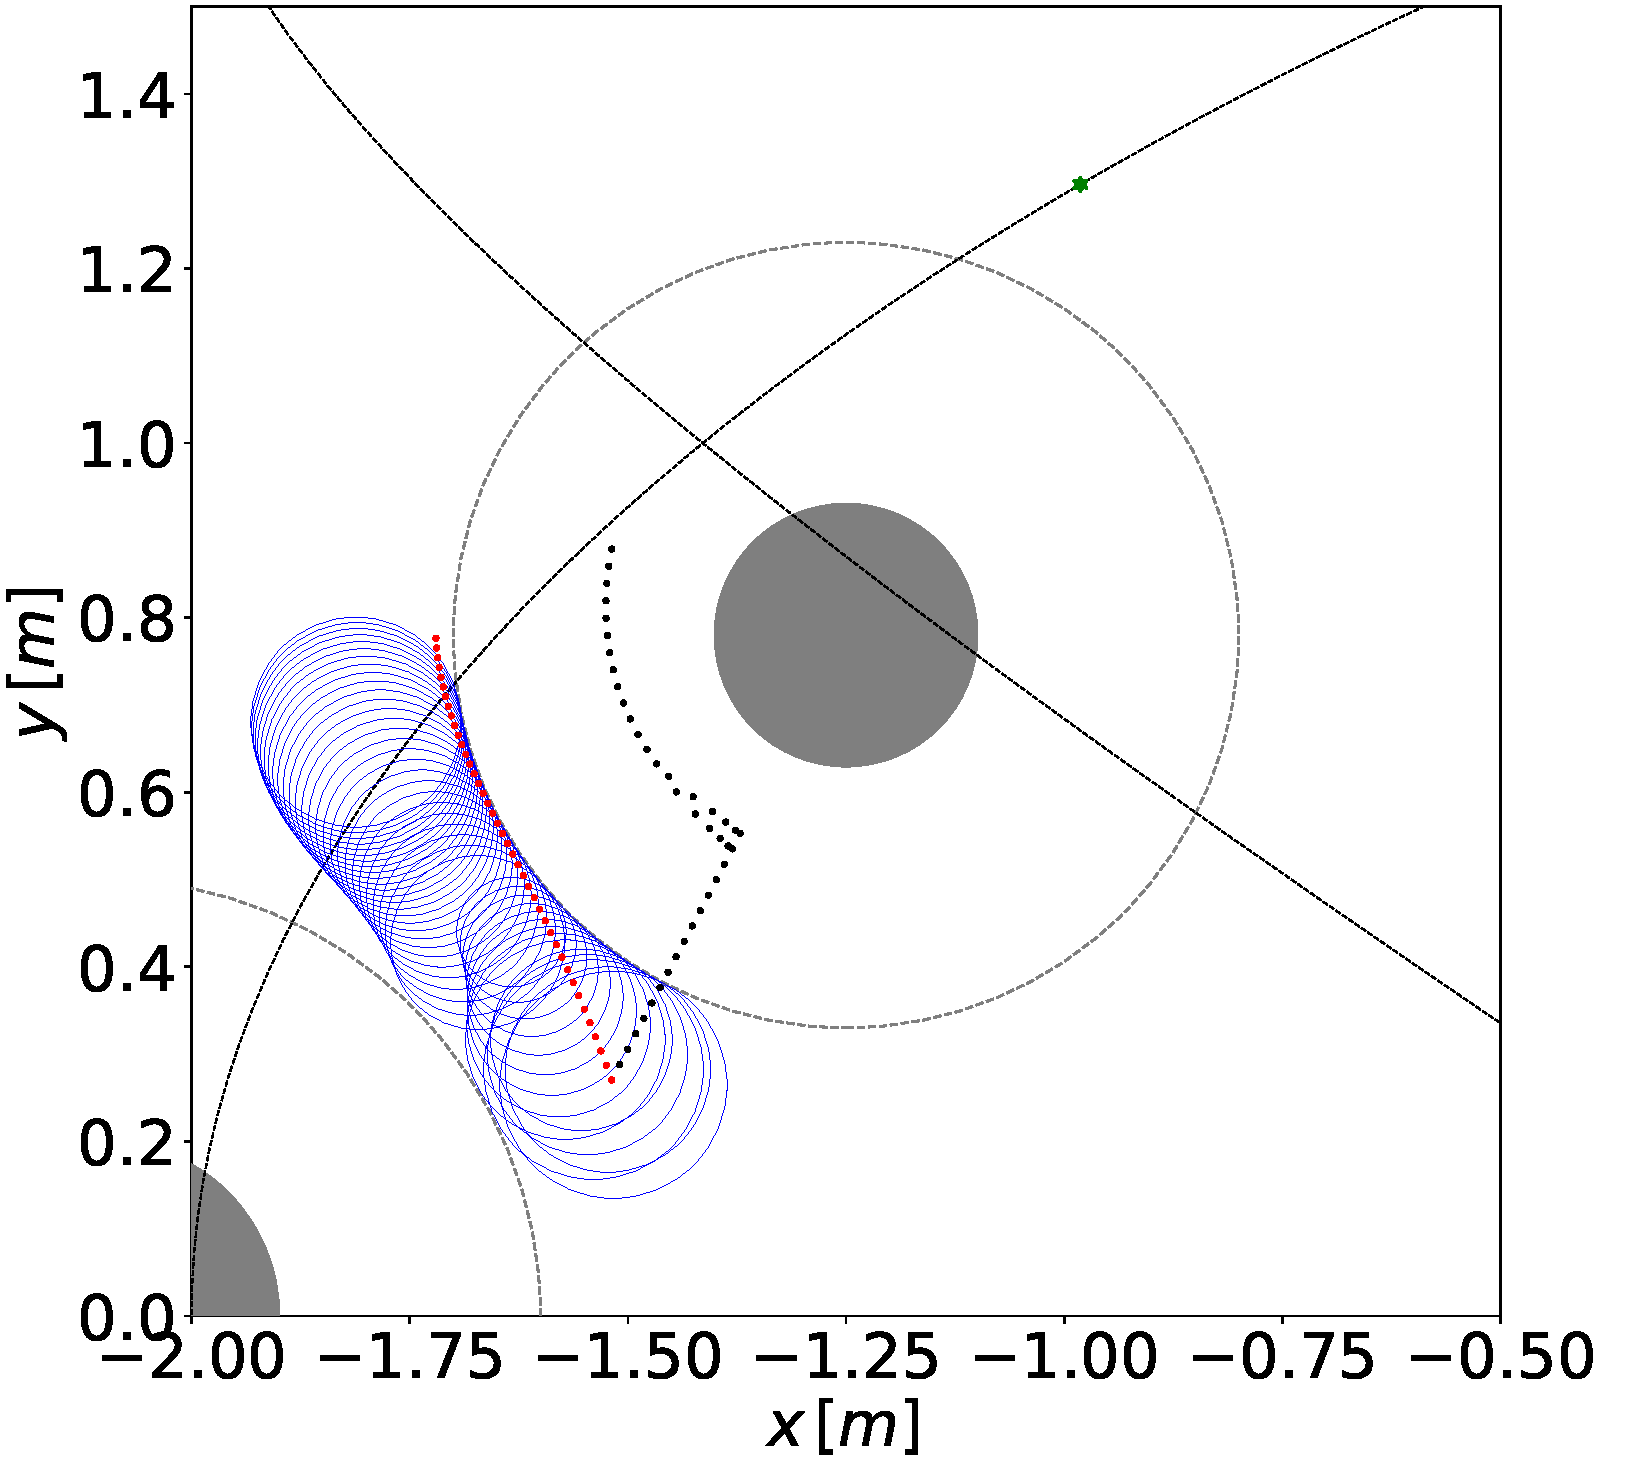
\includegraphics[width=0.32\linewidth]{Figures/Obstacle avoidance/Safe NMPC/example_ciao_circles_7.pdf}}
    \subfigure[Wider traversal between obstacles.]{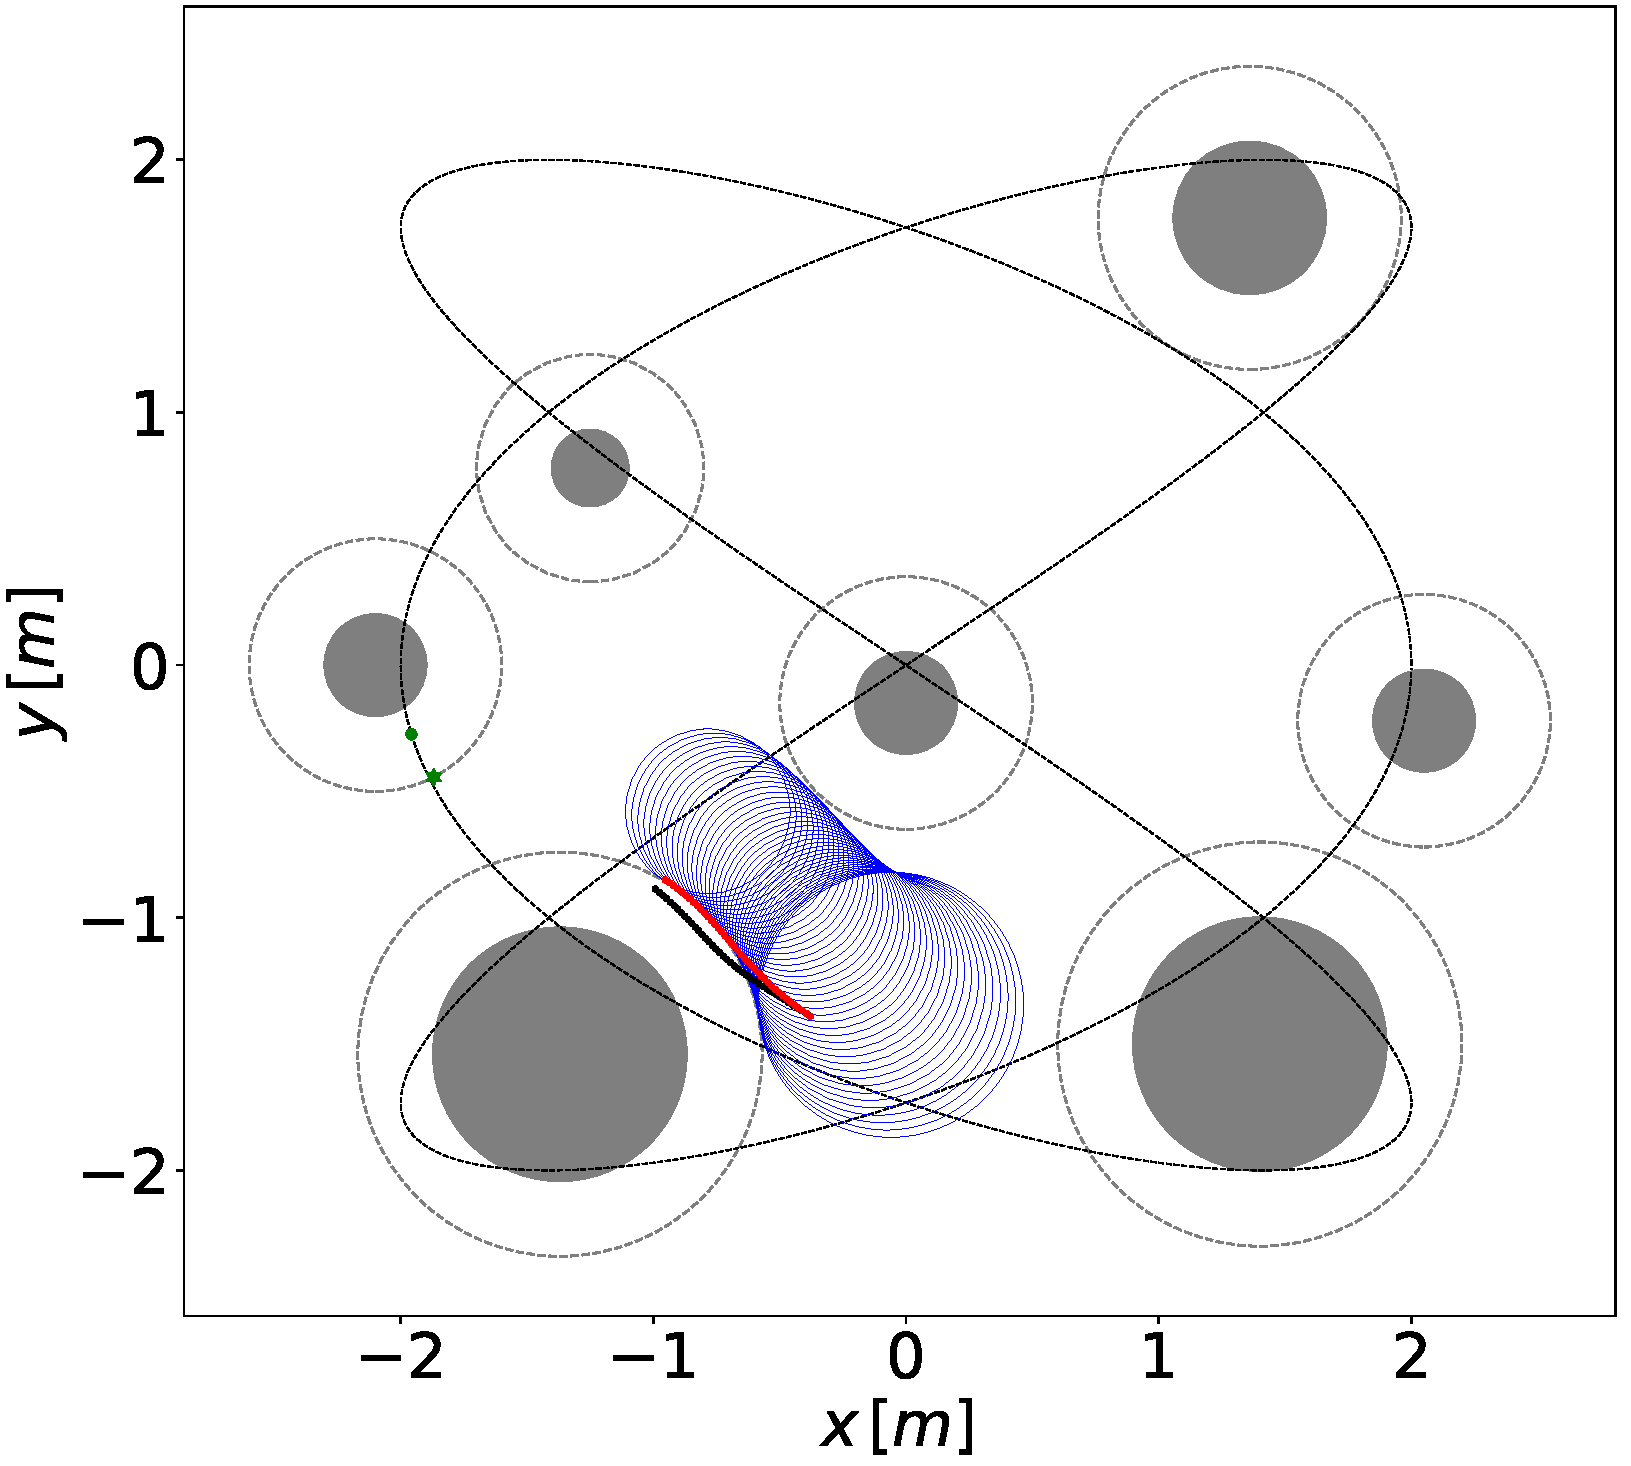
\includegraphics[width=0.32\linewidth]{Figures/Obstacle avoidance/Safe NMPC/example_ciao_circles_6.pdf}}
  \end{subfigmatrix}
  \caption{Size of safe balls (\textcolor{blue}{blue}) along optimal position horizon for solver $(1)$ on some situations. Reference position is marked in blacks dots, whereas the position horizon is marked by \textcolor{red}{red dots}. }
  \label{fig:safeballsexamplessolver1}
\end{figure}

The top left picture shows that when the mobile robot is far from the closest obstacle, its safe balls are big. The picture on its right depicts a situation where the last horizon node gets stucks because the reference end tip matches a quasi-static projected target on free space, that will begin to move when the original target moves deeper into the obstacle. The top right picture presents a situation where the safe balls size decrease as the mobile robot is moving between obstacles, where the safe area is small. As expected, the safe balls decrease as the horizon progressily enters this \textit{tunnel}.

The bottom left picture denotes an event where the mobile robot turns around, instead of circling the obstacle. As the target is too far ahead, the potential field redirects the reference. As a result of that, the optimal position horizon abruptly changes its course. The bottom middle picture depicts an high cost event. The fact that the horizon can't match the reference already introduces significant cost due to the safety constraints. However, a considerable higher cost comes to light as the reference contains back and forth segments because it crosses a local minimum position of the potential field. This \textit{bug} introduces significant heading differences between reference nodes, which breaks the assumption that the reference should be smooth. As a consequence of that, the solver is confused by the sudden yaw changes and the optimal solution degrades. Lastly, a wider traversal between obstacles is shown.

Similarly to the recorded position along the reference tracking tour in figure \ref{fig:pathtrackingsafeocp}, the position horizon is also at the safe space border whenever needed, so that it is closer to the reference path.

A video\footnote{Results of the safe one-stage \acrshort{ocp} real-time with solver $(1)$: \texttt{\url{https://youtu.be/xHckwLaS_dQ}} (accessed on 14 of February 2026)} was prepared to showcase the results of this chapter. The results rendered on that video were generated with solver $(1)$, under the same parameters that generated the results of this subsection.

% ----------------------------------------------------------------------
%\subsection{Figures}
%\label{subsection:figures}
%
%Insert your section material and possibly a few figures...
%
%Make sure all figures presented are referenced in the text!
%
%The caption should appear below the figure.

% ----------------------------------------------------------------------
%\subsubsection{Images}
%\label{subsection:images}
%
%\begin{figure}[!htb]
%  \centering
%  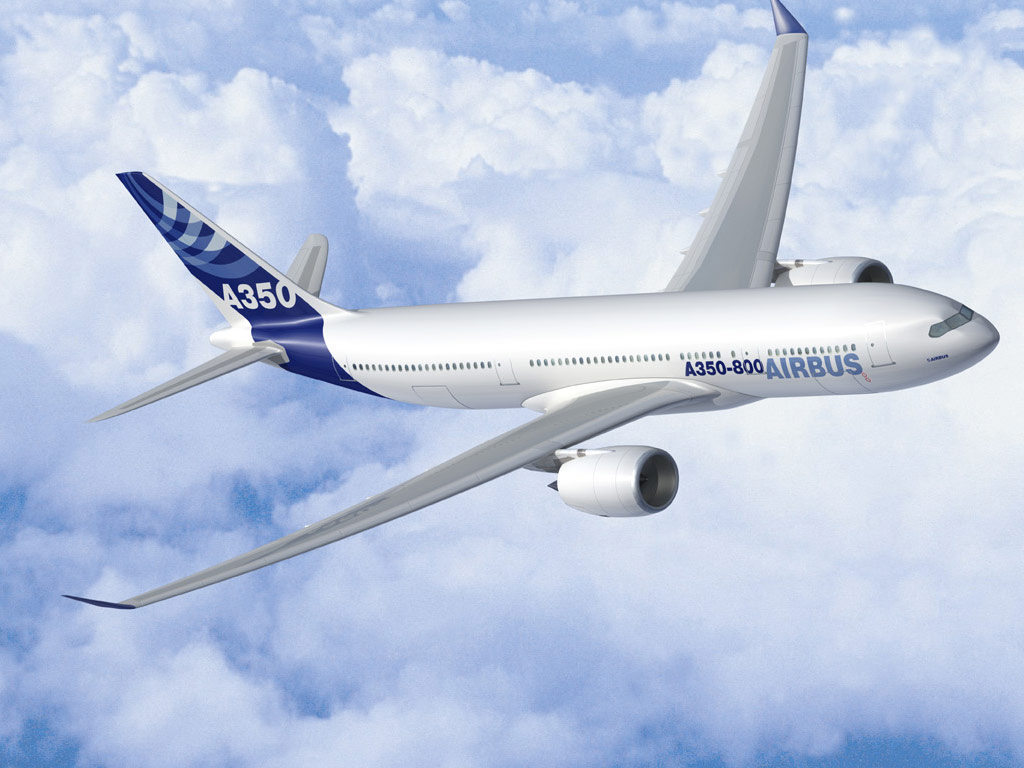
\includegraphics[width=0.25\textwidth]{Figures/Airbus_A350.jpg}
%  \caption[Caption for figure in TOC.]{Caption for figure.}
%  \label{fig:airbus1}
%\end{figure}
%
%\begin{figure}[!htb]
%  \begin{subfigmatrix}{2}
%    \subfigure[Airbus A320]{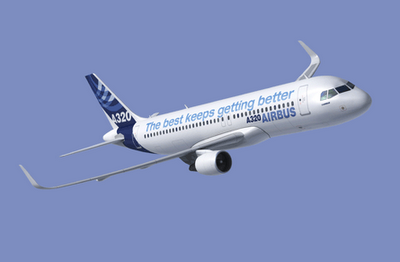
\includegraphics[width=0.49\linewidth]{Figures/Airbus_A320_sharklets.png}}
%    \subfigure[Bombardier CRJ200]{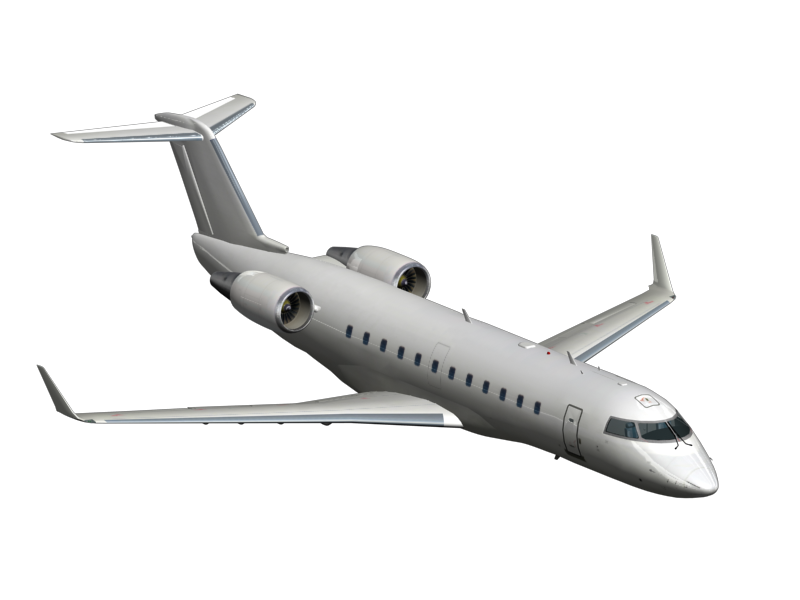
\includegraphics[width=0.49\linewidth]{Figures/Bombardier_CRJ200.png}}
%  \end{subfigmatrix}
%  \caption{Some aircrafts.}
%  \label{fig:aircrafts}
%\end{figure}
%
%Make reference to Figures~\ref{fig:airbus1} and \ref{fig:aircrafts}.
%
%By default, the supported file types are {\it .png,.pdf,.jpg,.mps,.jpeg,.PNG,.PDF,.JPG,.JPEG}.
%
%See \url{http://mactex-wiki.tug.org/wiki/index.php/Graphics_inclusion} for adding support to other extensions.


% ----------------------------------------------------------------------
%\subsubsection{Drawings}
%\label{subsection:drawings}
%
%Insert your subsection material and for instance a few drawings...
%
%The schematic illustrated in Fig.\ref{fig:algorithm} can represent some sort of algorithm.
%
%\begin{figure}[!htb]
%  \centering
%  \scriptsize
%%  \footnotesize 
%%  \small
%  \setlength{\unitlength}{0.9cm}
%  \begin{picture}(8.5,6)
%    \linethickness{0.3mm}
%
%    \put(3,6){\vector(0,-1){1}}
%    \put(3.5,5.4){$\bf \alpha$}
%    \put(3,4.5){\oval(6,1){}}
%    %\put(0,4){\framebox(6,1){}}
%    \put(0.3,4.4){Grid Generation: \quad ${\bf x} = {\bf x}\left({\bf \alpha}\right)$}
%
%    \put(3,4){\vector(0,-1){1}}
%    \put(3.5,3.4){$\bf x$}
%    \put(3,2.5){\oval(6,1){}}
%    %\put(0,2){\framebox(6,1){}}
%    \put(0.3,2.4){Flow Solver: \quad ${\cal R}\left({\bf x},{\bf q}\left({\bf x}\right)\right) = 0$}
%
%    \put(6.0,2.5){\vector(1,0){1}}
%    \put(6.4,3){$Y_1$}
%
%    \put(3,2){\vector(0,-1){1}}
%    \put(3.5,1.4){$\bf q$}
%    \put(3,0.5){\oval(6,1){}}
%    %\put(0,0){\framebox(6,1){}}
%    \put(0.3,0.4){Structural Solver: \quad ${\cal M}\left({\bf x},{\bf q}\left({\bf x}\right)\right) = 0$}
%
%    \put(6.0,0.5){\vector(1,0){1}}
%    \put(6.4,1){$Y_2$}
%
%    %\put(7.8,2.5){\oval(1.6,5){}}
%    \put(7.0,0){\framebox(1.6,5){}}
%    \put(7.1,2.5){Optimizer}
%    \put(7.8,5){\line(0,1){1}}
%    \put(7.8,6){\line(-1,0){4.8}}
%  \end{picture}
%  \caption{Schematic of some algorithm.}
%  \label{fig:algorithm}
%\end{figure}
%
%
%% ----------------------------------------------------------------------
%\subsection{Equations}
%\label{subsection:equations}
%
%Equations can be inserted in different ways.
%
%The simplest way is in a separate line like this
%
%\begin{equation}
%  \frac{{\rm d} q_{ijk}}{{\rm d} t} + {\cal R}_{ijk}({\bf q}) = 0 \,.
%\label{eq:ode}
%\end{equation}
%
%If the equation is to be embedded in the text. One can do it like this ${\partial {\cal R}}/{\partial {\bf q}}=0$.
%
%It may also be split in different lines like this
%
%\begin{eqnarray}
%  {\rm Minimize}   && Y({\bf \alpha},{\bf q}({\bf \alpha}))            \nonumber           \\
%  {\rm w.r.t.}     && {\bf \alpha} \,,                                 \label{eq:minimize} \\
%  {\rm subject~to} && {\cal R}({\bf \alpha},{\bf q}({\bf \alpha})) = 0 \nonumber           \\
%                   &&       C ({\bf \alpha},{\bf q}({\bf \alpha})) = 0 \,. \nonumber
%\end{eqnarray}
%
%It is also possible to use subequations. Equations~(\ref{eq:continuity}), (\ref{eq:momentum}) and (\ref{eq:energy}) form the Naver--Stokes equations~(\ref{eq:NavierStokes}).
%\begin{subequations}
%    \begin{equation}
%    \frac{\partial \rho}{\partial t} + \frac{\partial}{\partial x_j}\left( \rho u_j \right) = 0 \,,
%    \label{eq:continuity}
%    \end{equation}
%    \begin{equation}
%    \frac{\partial}{\partial t}\left( \rho u_i \right) + \frac{\partial}{\partial x_j} \left( \rho u_i u_j + p \delta_{ij} - \tau_{ji} \right) = 0, \quad i=1,2,3 \,,
%    \label{eq:momentum}
%    \end{equation}
%    \begin{equation}
%        \frac{\partial}{\partial t}\left( \rho E \right) + \frac{\partial}{\partial x_j} \left( \rho E u_j + p u_j - u_i \tau_{ij} + q_j \right) = 0 \,.
%    \label{eq:energy}
%    \end{equation}
%\label{eq:NavierStokes}%
%\end{subequations}
%
%
%% ----------------------------------------------------------------------
%\subsection{Tables}
%\label{section:tables}
%
%Insert your subsection material and for instance a few tables...
%
%Make sure all tables presented are referenced in the text!
%
%The caption should appear above the table.
%
%Follow some guidelines when making tables:
%
%\begin{itemize}
%  \item Avoid vertical lines
%  \item Avoid “boxing up” cells, usually 3 horizontal lines are enough: above, below, and after heading
%  \item Avoid double horizontal lines
%  \item Add enough space between rows
%\end{itemize}
%
%\begin{table}[!htb]
%  \caption[Table caption shown in TOC.]{Table caption.}
%  \label{tab:aeroCoeff}
%  \renewcommand{\arraystretch}{1.2} % more space between rows
%  \centering
%  \begin{tabular}{lccc}
%    \toprule
%    Model           & $C_L$ & $C_D$ & $C_{M y}$ \\
%    \midrule
%    Euler           & 0.083 & 0.021 & -0.110    \\
%    Navier--Stokes  & 0.078 & 0.023 & -0.101    \\
%    \bottomrule
%  \end{tabular}
%\end{table}
%
%Make reference to Tab.\ref{tab:aeroCoeff}.
%
%Tables \ref{tab:memory} and \ref{tab:multipleColumns} are examples of tables with merging columns:
%
%\begin{table}[!htb]
%  \caption{Memory usage comparison (in MB).}
%  \label{tab:memory}
%  \renewcommand{\arraystretch}{1.2} % more space between rows
%  \centering
%  \begin{tabular}[]{lrr}
%    \toprule
%                & \multicolumn{2}{c}{\underline{Virtual memory [MB]}} \\
%                & Euler       & Navier--Stokes \\
%    \midrule
%      Wing only &  1,000      &    2,000       \\
%      Aircraft  &  5,000      &   10,000       \\
%      (ratio)   & $5.0\times$ & $5.0\times$    \\
%    \bottomrule
%  \end{tabular}
%\end{table}
%
%\begin{table}[!htb]
%  \caption{Another table caption.}
%  \label{tab:multipleColumns}
%  \centering
%  \renewcommand{\arraystretch}{1.2} % more space between rows
%  \begin{tabular}{@{}rrrrcrrr@{}} % remove space to the vertical edges @{}...@{}
%    \toprule
%      & \multicolumn{3}{c}{$w = 2$} & \phantom{abc} & \multicolumn{3}{c}{$w = 4$} \\
%    \cmidrule{2-4}
%    \cmidrule{6-8}
%      & $t=0$ & $t=1$ & $t=2$ && $t=0$ & $t=1$ & $t=2$ \\
%    \midrule
%      $dir=1$
%      \\
%      $c$ &  0.07 &  0.16 &  0.29 &&  0.36 &  0.71 &   3.18 \\
%      $c$ & -0.86 & 50.04 &  5.93 && -9.07 & 29.09 &  46.21 \\
%      $c$ & 14.27 &-50.96 &-14.27 && 12.22 &-63.54 &-381.09 \\
%      $dir=0$
%      \\
%      $c$ &  0.03 &  1.24 &  0.21 &&  0.35 & -0.27 &  2.14 \\
%      $c$ &-17.90 &-37.11 &  8.85 &&-30.73 & -9.59 & -3.00 \\
%      $c$ &105.55 & 23.11 &-94.73 &&100.24 & 41.27 &-25.73 \\
%    \bottomrule
%  \end{tabular}
%\end{table}
%
%An example with merging rows can be seen in Tab.\ref{tab:multipleRows}.
%
%\begin{table}[!htb]
%  \caption{Yet another table caption.}
%  \label{tab:multipleRows}
%  \renewcommand{\arraystretch}{1.2} % more space between rows
%  \centering
%  \begin{tabular}{ccccc}
%    \toprule
%      \multirow{2}{*}{ABC} & \multicolumn{4}{c}{header} \\
%      \cmidrule{2-5} & 1.1 & 2.2 & 3.3 & 4.4 \\
%    \midrule
%      \multirow{2}{*}{IJK} & \multicolumn{2}{c}{\multirow{2}{*}{group}} & 0.5 & 0.6 \\
%      \cmidrule{4-5}       & \multicolumn{2}{c}{}                       & 0.7 & 1.2 \\
%    \bottomrule
%  \end{tabular}
%\end{table}
%
%If the table has too many columns, it can be scaled to fit the text widht, as in Tab.\ref{tab:scale}.
%\begin{table}[!htb]
%  \caption{Very wide table.}
%  \label{tab:scale}%
%  \renewcommand{\arraystretch}{1.2} % more space between rows
%  \centering
%  \resizebox*{\textwidth}{!}{%
%    \begin{tabular}[]{lcccccccccc}
%      \toprule
%        Variable &  a  &  b  &  c  &  d  &  e  &  f  &  g  &  h  &  i  &  j  \\
%      \midrule
%        Test 1   &  10,000 &  20,000 &  30,000 &  40,000 &  50,000 &  60,000 &  70,000 &  80,000 &  90,000 & 100,000 \\
%        Test 2   &  20,000 &  40,000 &  60,000 &  80,000 & 100,000 & 120,000 & 140,000 & 160,000 & 180,000 & 200,000 \\
%      \bottomrule
%    \end{tabular}
%  }%
%\end{table}
%
%
%% ----------------------------------------------------------------------
%\subsection{Mixing}
%\label{section:mixing}
%
%If necessary, a figure and a table can be put side-by-side as in Fig.\ref{fig:side_by_side}
%
%\begin{figure}[!htb]
%  \begin{minipage}[b]{0.60\linewidth}
%    \centering
%    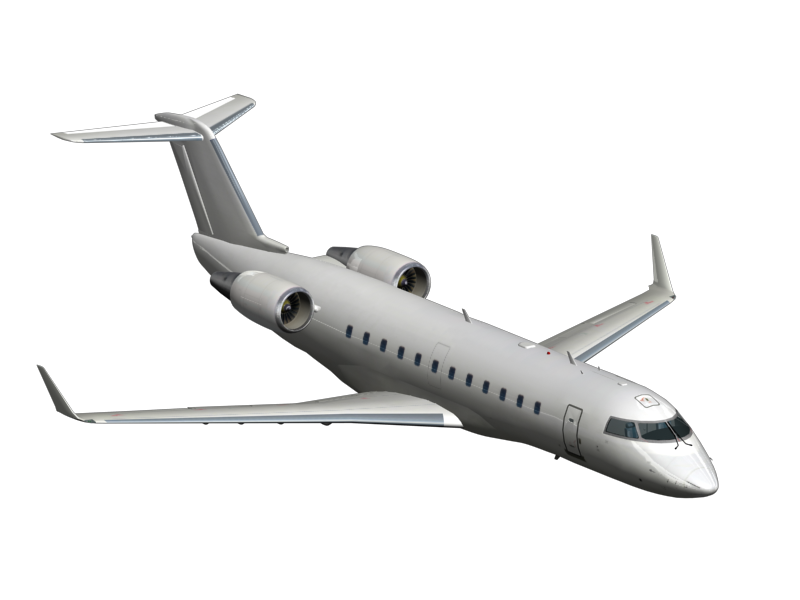
\includegraphics[width=\linewidth]{Figures/Bombardier_CRJ200}
%  \end{minipage}%
%  \begin{minipage}[b]{0.30\linewidth}
%    \centering
%    \begin{tabular}[b]{lll}
%      \toprule
%        \multicolumn{3}{c}{Legend} \\
%      \midrule
%        A & B & C \\
%        0 & 0 & 0 \\
%        0 & 1 & 0 \\
%        1 & 0 & 0 \\
%        1 & 1 & 1 \\
%      \bottomrule
%    \end{tabular}
%    \vspace{5em}
%  \end{minipage}
%\caption{Figure and table side-by-side.}
%\label{fig:side_by_side}
%\end{figure}

